
\chapter{Evaluation}
\label{sec:evaluation}
In this chapter, we explain in detail our experimental setup and discuss the extracted results. Afterwards we examine the impact of the configuration parameters, the legal entity of the TPDs, their geographical location, as well as the position of the FPDs in the Alexa rank on the achieved privacy level.

\section{Experimental setup}
In this subsection, we outline the experimental setup and configuration. To this end we make use of Lightbeam (a Firefox browser extension) in order to build the graph $G$.

\subsection{Lightbeam first party heuristics}
The distinction between FPRs and TPRs is crucial in our attempt to precisely quantify the filtering capability for each adblocker, since they define the exact topology of the derived graph $G$.

Related work~\cite{ruffel2015} has adopted Lightbeam to capture the TPRs. Nonetheless, Lightbeam does not always know the exact source of each HTTP request sent from our browser. As a consequence, it implements heuristics to determine the source domain that a request is initiated from and afterwards classifies it accordingly as a FPR or a TPR.

This classification, however, is not always in accordance with our definitions of FPR and TPR, as introduced in Chapter~\ref{sec:privacy_metrics}. By examining the request logs after a complete crawl cycle and comparing the estimated source to the actual visited domain, two types of false-positive cases (Table~\ref{table:false_positive_examples}) arise:

\begin{itemize}
\item \textbf{Unrecognized TPRs:} The request is mistakenly considered to be a FPR according to the Lightbeam heuristics, this way ``hiding'' a TPR edge from the graph.
\item \textbf{Misclassified TPRs:} The request is correctly found to be a TPR, but not for the correct FPD node, i.e.\ the one corresponding to the actually crawled domain. The inaccuracy introduced to the graph results from the potential introduction of a bogus FPD node, as well as the false number of TPR edges starting from the correct and the bogus FPD nodes.
\end{itemize}

As results from the experimental evaluation on the data of one full crawl cycle (1000 visited first parties) and 12 different browser profiles, the misclassified and unrecognized TPRs make up for 2.0\%-12.0\% and 4.0\%-11.0\% of the total requests, depending on the respective browser profiles that we define further.

\begin{table}
\centering
\footnotesize
\begin{tabular}{|c|c c c|}

\hline
& Visited Domain & Estimated Source & Target \\
\hline
Recognized & wp.pl & wp.pl & facebook.com \\
Misclassified & wp.pl & facebook.com & fbcdn.net \\
Unrecognized & wp.pl & facebook.com & facebook.com \\
\hline
\end{tabular}
\caption{Examples of misclassified and unrecognized TPRs}
\label{table:false_positive_examples}
\end{table}

\subsection{Evaluation Parameters}

In the following we define the different adblocker configurations and which URLs we evaluate on a daily basis.

\paragraph{Browser profiles}
\label{sec:browser_profiles}
In order to compare the filtering performance of different adblockers, as well as the influence of different browser settings on their ad-blocking efficiency, we create 12 browser profiles, $U$, each of which is defined as a combination of the following parameters (Table~\ref{table:browser_profiles}):

\begin{itemize}
 \item Ad-blocker installed
 \item Block policy: maximum or default protection\footnote{Ghostery's policy is configured through the selection of trackers to be blocked from a pre-defined list. By default no tracker is blocked and in maximum-protection settings, all trackers are blocked.
 
 AdblockPlus' policy is defined by the activation of publicly available blacklists. By default, ``EasyList'' is activated, whilst in maximum-protection settings, the activated blacklists are ``EasyList'', ``EasyList China'', ``EasyPrivacy'' and ``Peter Lowe's List''.}
 \item Mobile or Desktop User Agent
 \item Do Not Track (DNT) header enabled
\end{itemize}

\paragraph{Crawled URLs}
\label{sec:crawled_urls}
An appropriate criterion for the evaluation of an adblocker is its filtering performance in the most frequent case. Consequently, it is plausible to test its efficiency for instance on the \textit{500 domains with the highest incoming web traffic}. Considering the top-visited domains, however, would imply the risk of favoring an adblocker optimized to perform better for a certain group of websites, eventually biasing the experimental results. We therefore extend our URL sample set with another \textit{500 uniformly-selected domains} among the top 1 million most-visited domains from the Alexa Traffic Rank. The sample set $S$ of 1000 URLs is stored and kept unchanged throughout the evaluation period, so as to de-correlate any variations of the results between two different days.

Since nowadays most web applications are based on asynchronous calls to fetch data, it is insufficient to wait for the DOM to finish rendering to record all resource requests sent from the website to any first or third parties. To collect the complete data and better simulate the common user browsing behavior, our crawler therefore waits 20 seconds on each website of our sample set $S$ and records any requests sent, before closing and proceeding to the next domain. Additionally, we modify \textit{Lightbeam} to account for the currently visited first-party --- and we thus do not rely on Lightbeam's heuristics.

Last but not least, in order to decouple the experimental conditions from the influence of any time- or location-related effects ---i.e.\ variations of the served content, locale-based personalization--- all browser profiles $U$ execute the same crawling routine simultaneously, whilst running on the same machine, thus behind the same IP address, Browser and Operating System. However, some of the instances are configured to send their requests with a User-Agent HTTP header that corresponds to a mobile device (iPhone with iOS 6), in order to extend our observations for mobile users.

\section{Experimental Results}
In this section, we present our experimental results. We use the following conventions for each browser profile $U$ (cf. Figure~\ref{fig:metrics_without_entities}):
\begin{itemize}
 \item The \textit{color} denotes the adblocker installed.
 \item The \textit{line width} indicates the protection degree ---i.e.\ default, maximum protection or DNT header.
 \item Profiles with Mobile User Agent are plotted in \textit{dashed lines}.
\end{itemize}
The data collected for browser profile $U$ on a specific date correspond to a different graph $G$. The plot legends corresponding to each browser profile $U$ are described in Table~\ref{table:browser_profiles}.

  \begin{table*}
%   \centering
  \small
  \begin{adjustbox}{center}
  \begin{tabular}{|c|c c c c c|}
  \hline
  Browser Profile & Adblocker & Block Policy & DNT & User Agent & Legend \\
  \hline
  Ghostery\_Default & Ghostery & Default & No & Desktop  & {\color{red}\solidthinrule} \\
  Ghostery\_MaxProtection & Ghostery & Max & No & Desktop & {\color{red}\solidthickrule} \\
  Adblockplus\_Default & AdblockPlus & Default & No & Desktop & {\color{blue}\solidthinrule} \\
  Adblockplus\_MaxProtection & AdblockPlus & Max & No & Desktop & {\color{blue}\solidthickrule} \\
  NoAdblocker & None & - & No & Desktop & {\color{darkgreen}\solidthinrule} \\
  NoAdblocker\_DNT & None & - & Yes & Desktop & {\color{darkgreen}\solidthickrule} \\
  Ghostery\_Default\_MUA & Ghostery & Default & No & Mobile & {\color{red}\dashedthinrule} \\
  Ghostery\_MaxProtection\_MUA & Ghostery & Max & No & Mobile & {\color{red}\dashedthickrule} \\
  Adblockplus\_Default\_MUA & AdblockPlus & Default & No & Mobile & {\color{blue}\dashedthinrule} \\
  Adblockplus\_MaxProtection\_MUA & AdblockPlus & Max & No & Mobile & {\color{blue}\dashedthickrule} \\
  NoAdblocker\_MUA & None & - & No & Mobile & {\color{darkgreen}\dashedthinrule} \\
  NoAdblocker\_DNT\_MUA & None & - & Yes & Mobile & {\color{darkgreen}\dashedthickrule} \\
  \hline
  
  \end{tabular}
  \end{adjustbox}
  \caption{Overview of browser profiles examined}
  \label{table:browser_profiles}
  \end{table*}
  


\subsection{Mean FPD node degree, mean TPD node degree and graph density over time}
\label{sec:metrics_without_entities}
We now study the evaluation of the FPD node degree, the TPD node degree and the graph density over time. Recall that the node degree of a FPD indicates how many TPDs are loaded by this FPD. Accordingly, the degree of an TPD shows how many of the FPDs this TPD has access to.

We observe (Figure~\ref{fig:first_means}) that the browser profiles \textit{Ghostery\_Default} and \textit{NoAdblocker} have the worst filtering performance, since the first parties visited load the highest number of third-party domains. Similarly, Figure~\ref{fig:third_means} shows that for these browser profiles the third parties loaded have access to the highest mean number of first parties. Although we would expect that the use of an adblocker, such as Ghostery, should provide us with better results, a closer look at its initial settings shows that the adblocker functions as a third-party tracker that does not block any third parties by default, unless configured appropriately. The metric has a consistently but only slightly lower value for the profile \textit{NoAdblocker\_DNT}.

The browser profiles with the same settings but with a Mobile User Agent (\textit{Ghostery\_\allowbreak Default\_\allowbreak MUA}, \textit{NoAdblocker\_\allowbreak MUA} and \textit{NoAdblocker\_\allowbreak DNT\_\allowbreak MUA}) have a mean FPD node degree and a mean TPD node degree lower by roughly 15\%. Comparing the three browser profiles with each other though, we see that their relative order remains unaltered.

The mean FPD and TPD node degrees when AdblockPlus is used with its default settings (\textit{Adblockplus\_\allowbreak Default} and \textit{Adblockplus\_\allowbreak Default\_\allowbreak MUA}) are significantly lower than the aforementioned worst cases, i.e. no adblocker or Ghostery at its default configuration.

Unsurprisingly, the browser profiles that filter the most third parties are those configured to a maximum protection level. We observe that the mean node degrees decrease by approximately 80\% compared to the default protection level. Ghostery moreover consistently performs better than AdblockPlus, when both are set to the maximum protection settings.

An inspection of the graph-density plot (Figure~\ref{fig:density}) for each of the profiles tested yields similar results: The profiles \textit{Ghostery\_\allowbreak Default} and \textit{NoAdblocker} present the worst filtering efficiency, setting the DNT header brings a slight amelioration, the usage of AdblockPlus even with default settings comes with considerably better results, whilst the best filtering performance is achieved by the profile \textit{Ghostery\_\allowbreak MaxProtection} followed by \textit{Adblockplus\_\allowbreak MaxProtection}. Nonetheless, the use of Mobile User Agent seems now to deteriorate the graph density, although it improved the TPD node degree. We explain this behavior with the fact that from all of the third parties that were loaded under a Desktop User Agent, only the most popular ones are still loaded under a Mobile User Agent, i.e.\ the ones that have a higher chance of being requested by more FPDs, e.g. \texttt{doubleclick.net}. Henceforth, although the mean TPD node degree is lower for the Mobile User Agent, the absolute number of TPD nodes is also considerably lower compared to the Desktop User Agent, which leads to a higher graph density according to Formula~\ref{eq:density}, or equivalently a more connected graph.

Because, the User Agent however is not a privacy-related setting ---e.g. adblocker, protection level, DNT header--- the analysis of the filtering performance of a configuration does not involve the impact of this parameter on the achieved privacy level. As a consequence, the graph density still provides a valid metric for the evaluation and comparison of the filtering effectiveness of different privacy configurations.

Although all of the three metrics examined provide valid and accurate results regarding the performance of browser profiles with different privacy settings, they are not capable of discerning the differences between the profiles to the same extent. More precisely, suppose we want to compare the blocking capability of the profiles \textit{Ghostery\_\allowbreak Default} and \textit{Ghostery\_\allowbreak MaxProtection}. When the mean FPD node degree is used as a metric (Figure~\ref{fig:first_means}), the results we get with the maximum-protection settings are approximately 4.7 times better with respect to those we get with the default settings. Similarly, using as metrics the mean TPD node degree (Figure~\ref{fig:third_means}) and graph density (Figure~\ref{fig:density}), the results provided by \textit{Ghostery\_\allowbreak MaxProtection} are 3 and 2 times better, accordingly.
% Notwithstanding that the relative filtering performance of the browser profiles remained practically unaltered with the use of the different metrics, as illustrated above, the discrepancies between the results of the profiles are not always trivial to tell apart.
As a consequence, the mean TPD node degree is less suitable than the mean FPD node degree when profiles with finer efficiency differences are to be discerned, while their distignuishability weakens markedly further when the graph density is used as a metric.

  \begin{figure*}
   \centering
\subfloat[Mean FPD node degree]{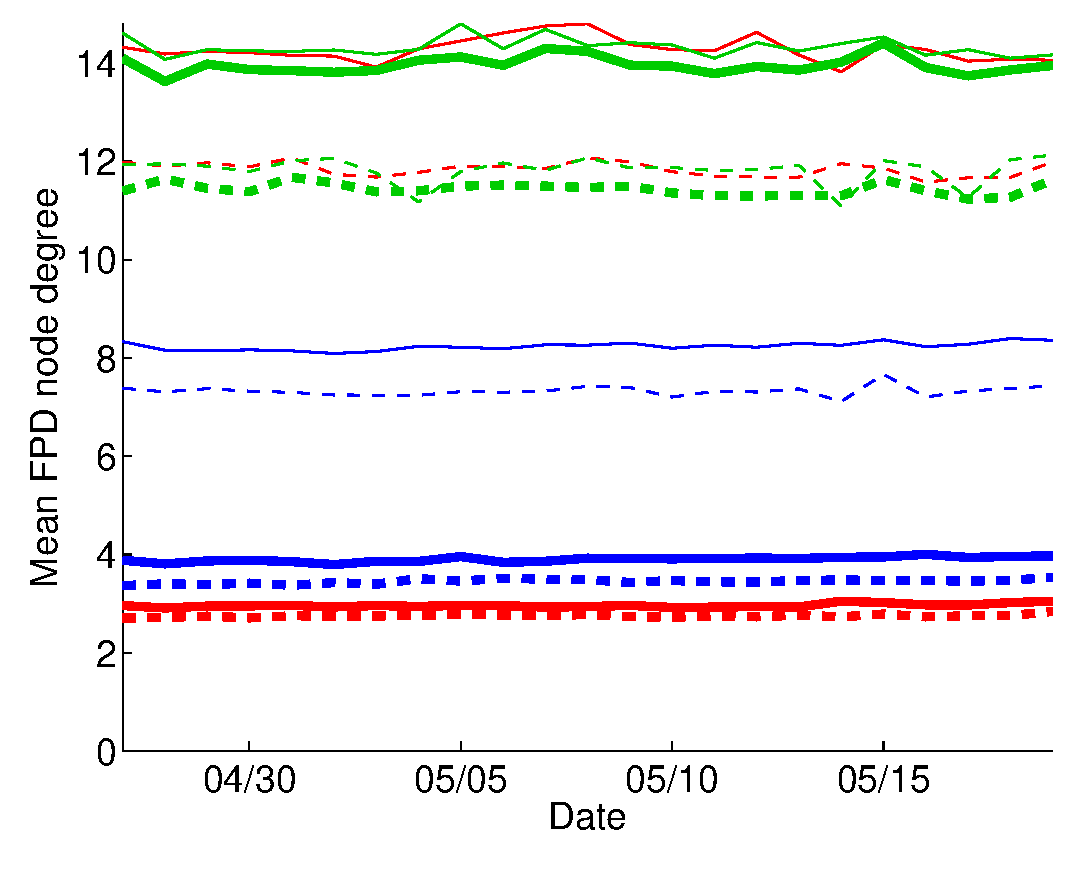
\includegraphics[width=.45\textwidth]{figures/first-means.eps}\label{fig:first_means}} \hfill
  \subfloat[Mean TPD node degree]{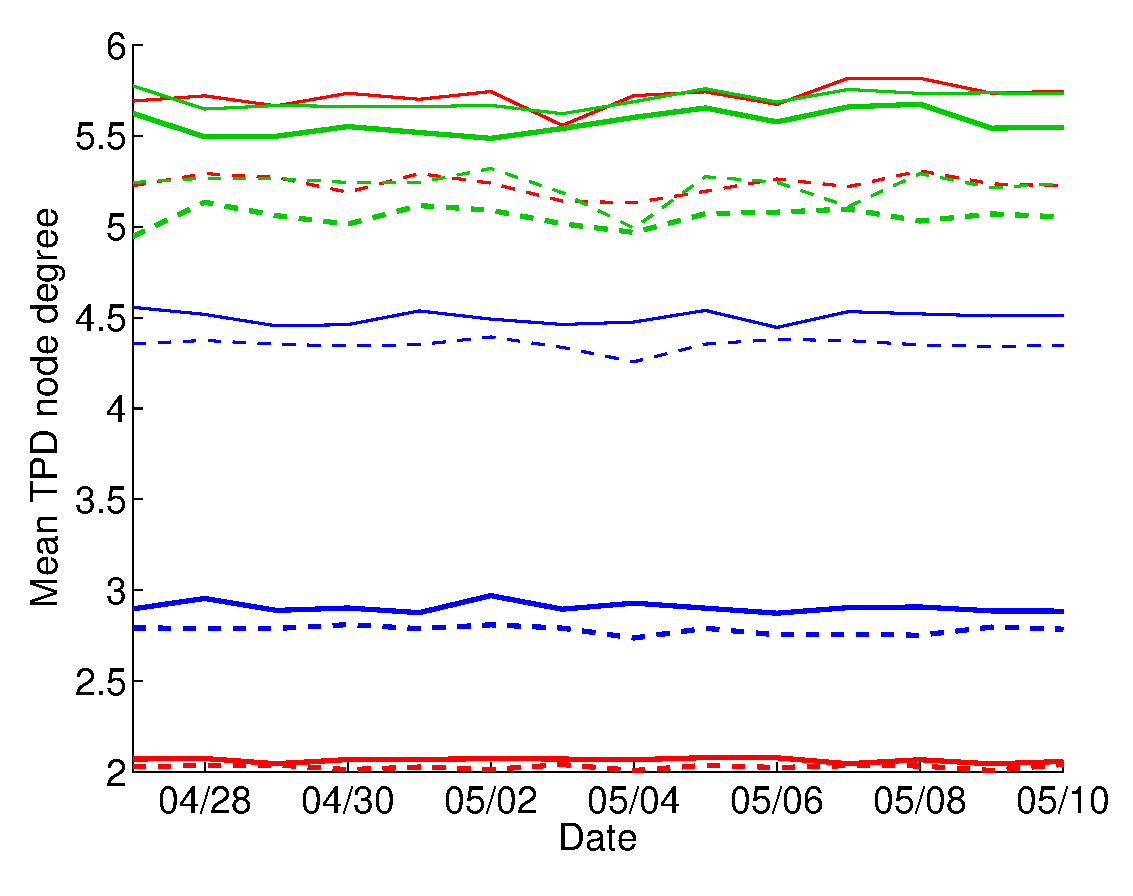
\includegraphics[width=.45\textwidth]{figures/third-means.eps}\label{fig:third_means}} \\
  \subfloat[Graph density]{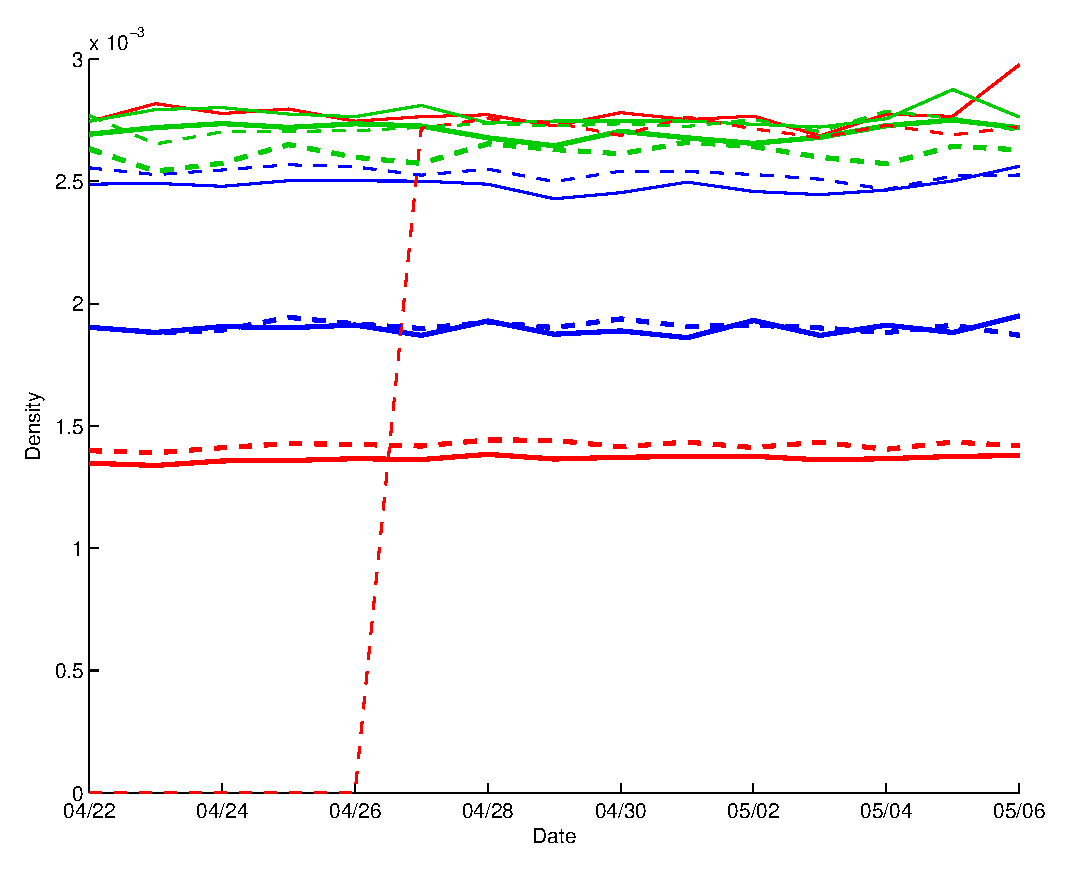
\includegraphics[width=.45\textwidth]{figures/density.eps}\label{fig:density}}

  \caption{Time evolution of graph metrics for all browser profiles}
  \label{fig:metrics_without_entities}
  \end{figure*}

\subsection{Mean value and standard deviation of FPD node degree over time}
Examining the cumulative distribution function (CDF) of the FPD node degree (Figures~\ref{fig:cdf_mean_first_node_degree},~\ref{fig:stdev_first_node_degree}) we can profile the extent to which the visited URLs are being tracked by third party domains. For each FPD we calculate the mean node degree across multiple days. Afterwards, we plot the probability $$P(\textnormal{FPD node degree} \leq X)$$ of a FPD node to have a mean degree less than $X$ or, equivalently, to load on average less than $X$ TPDs. A browser profile whose corresponding curve lies on the leftmost side of the graph is expected to have a lower mean FPD node degree which is equivalent to a better filtering performance in terms of privacy.

As results from Figure~\ref{fig:cdf_mean_first_node_degree}, 20\% of the visited domains (FPD nodes) load more than 20 third parties under the browser profiles \textit{Ghostery\_Default}, \textit{NoAdblocker} and \textit{NoAdblocker\_DNT}, hence presenting the worst performance. On the contrary, when Ghostery is used with maximum protection, the most TPDs are blocked and almost no FPD node has a mean node degree higher than 20.

\begin{figure}
 \centering
  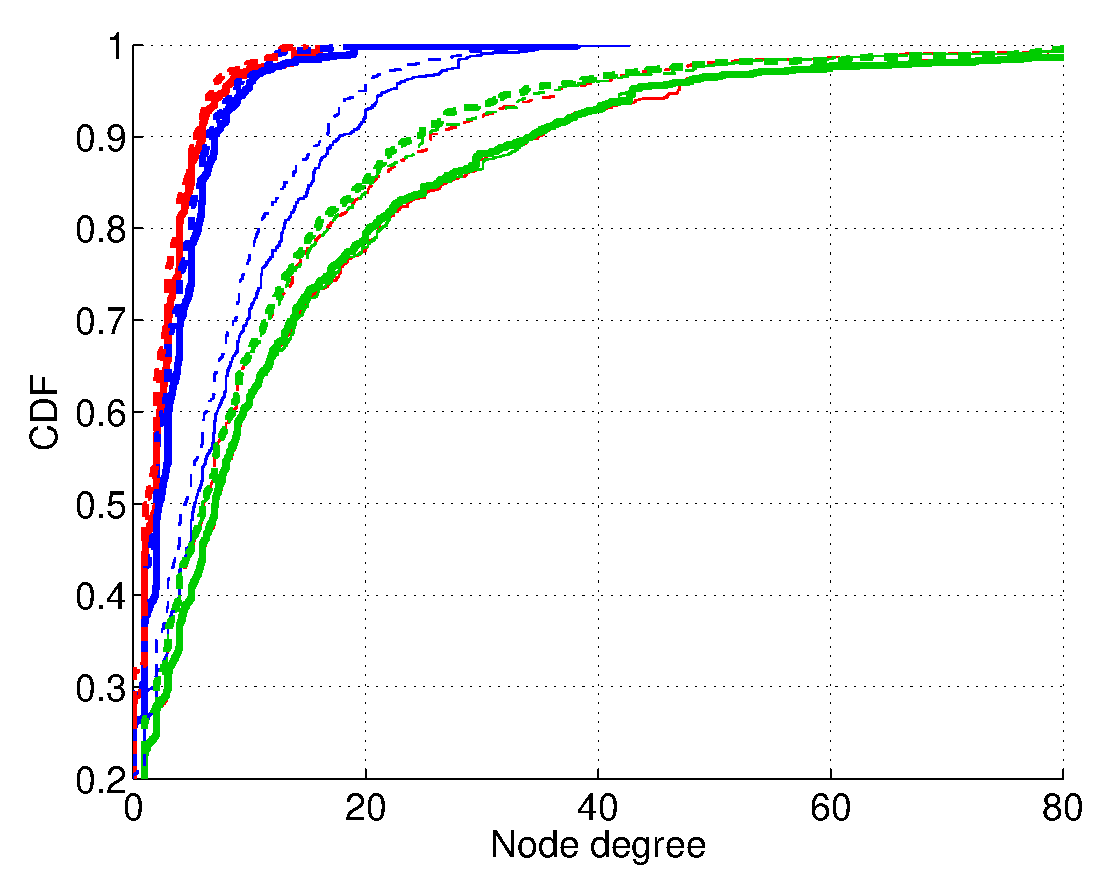
\includegraphics[width=.45\textwidth]{figures/cdf-scatterplot-means.eps}
  \caption{Mean FPD node degree across time for all browser profiles}
  \label{fig:cdf_mean_first_node_degree}
\end{figure}

\begin{figure*}
 \centering
 
 \subfloat[CDF for all 1000 visited sites and all browser profiles.]{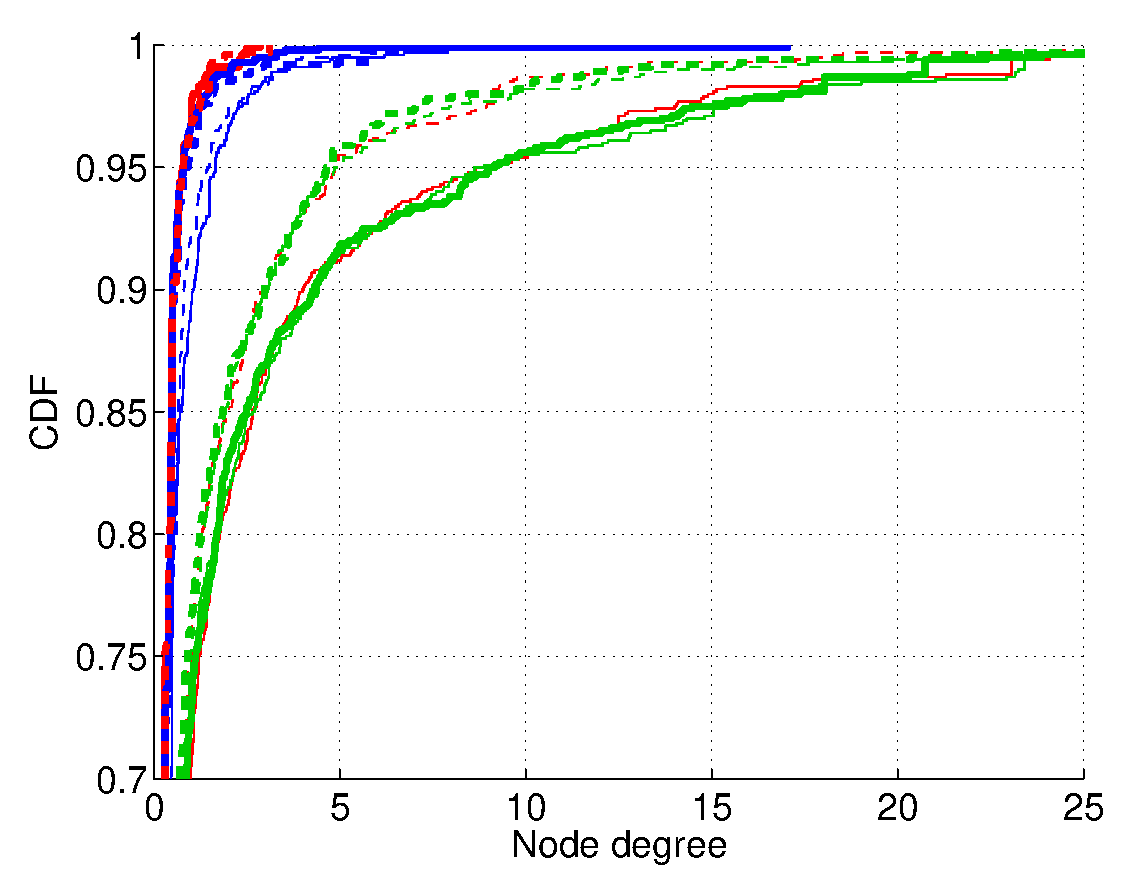
\includegraphics[width=.45\textwidth]{figures/cdf-scatterplot-stdev.eps}\label{fig:cdf_stdev_first_node_degree}} \hfill
 \subfloat[Scatterplot for the 500 top-ranked sites for browser profile \textit{NoAdblocker}.]{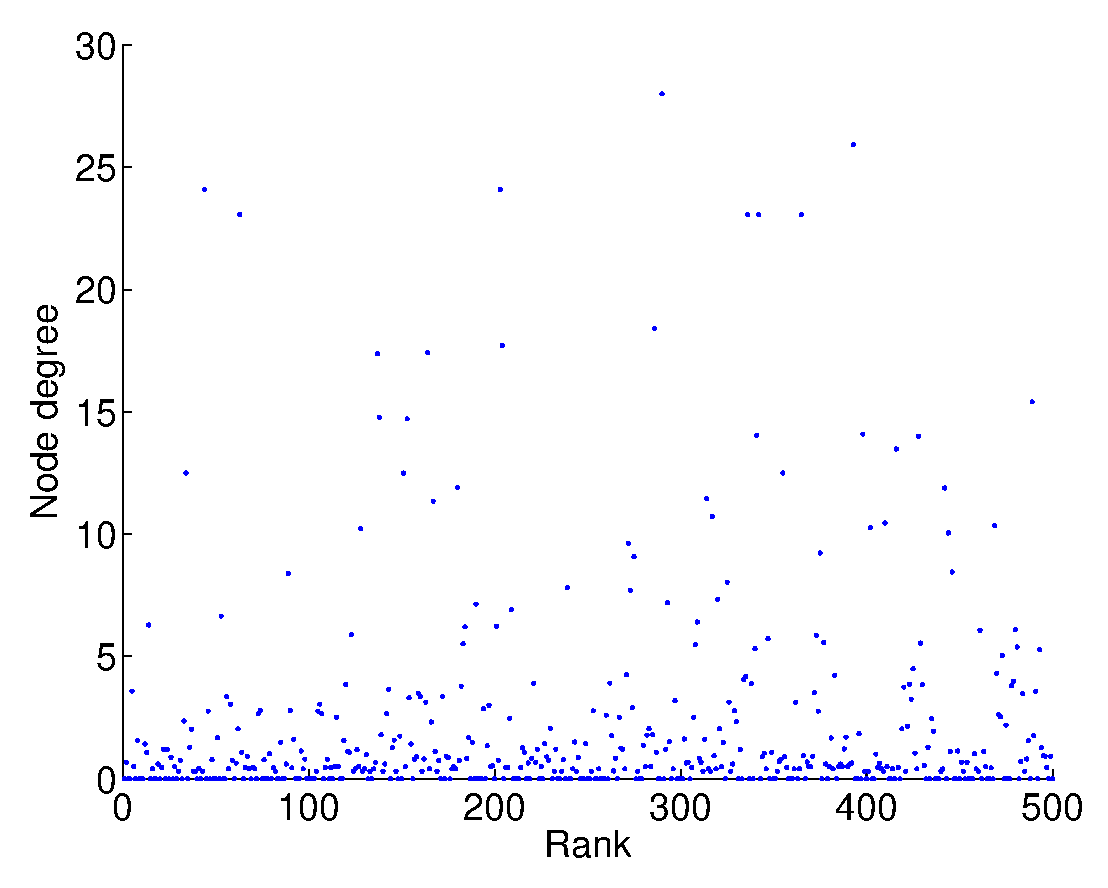
\includegraphics[width=.45\textwidth]{figures/scatterplot-stdev.eps}\label{fig:scatterplot-per-rank}}
 
 \caption{Standard deviation across time of FPD node degree}
 \label{fig:stdev_first_node_degree}
\end{figure*}

\subsection{CDF of FPD and TPD node degree}
In Figure~\ref{fig:cdf_first_third_node_degree} we visualize the FPD and TPD node degrees for a specific date and create the CDF of the two metrics. Although the results are in accord with the conclusions of the previous plots (cf. Figures~\ref{fig:metrics_without_entities},~\ref{fig:cdf_mean_first_node_degree},~\ref{fig:cdf_stdev_first_node_degree}), it is to be observed that the FPD node degree gives us a better discerning ability with respect to the TPD node degree for profiles with similar filtering performances confirming our observation in~\ref{sec:metrics_without_entities}.

For example, when comparing the blocking performance of \textit{Ghostery\_\allowbreak MaxProtection} and \textit{Adblockplus\_\allowbreak MaxProtection} based on the FPD node degree (Figure~\ref{fig:cdf-first-node-degree}), we observe that  the CDF curves for the two profiles coincide for $CDF \le 0.3$ and $d \le 1$, where $d$ the node degree. This means that 30\% of the FPD nodes for one browser profile has the exact same distribution as 30\% of the FPD nodes for the other browser profile and hence we cannot tell which one of the two presents a better filtering performance by examining only this part of the curve. However, for each value of node degree, $d > 1$, the browser profile \textit{Ghostery\_\allowbreak MaxProtection} has less FPD nodes that have a node degree as high as $d$ than the browser profile \textit{Adblockplus\_\allowbreak MaxProtection} has, which can be directly translated to a better filtering performance for the profile \textit{Ghostery\_\allowbreak MaxProtection}.

Accordingly, the better performance for the profile \textit{Ghostery\_\allowbreak MaxProtection} can be concluded similarly when we use the TPD node degree as a metric (Figure~\ref{fig:cdf-third-node-degree}). Nevertheless, the part where the two curves coincide ---and thence do not offer any comparative result--- is for $CDF \le 0.95$. As a consequence, to compare the performances of the two browser profiles, we have to examine a much smaller part of the curve, which leads to less clear conclusions.

  \begin{figure*}[!t]
  \centering
  \subfloat[FPD node degree]{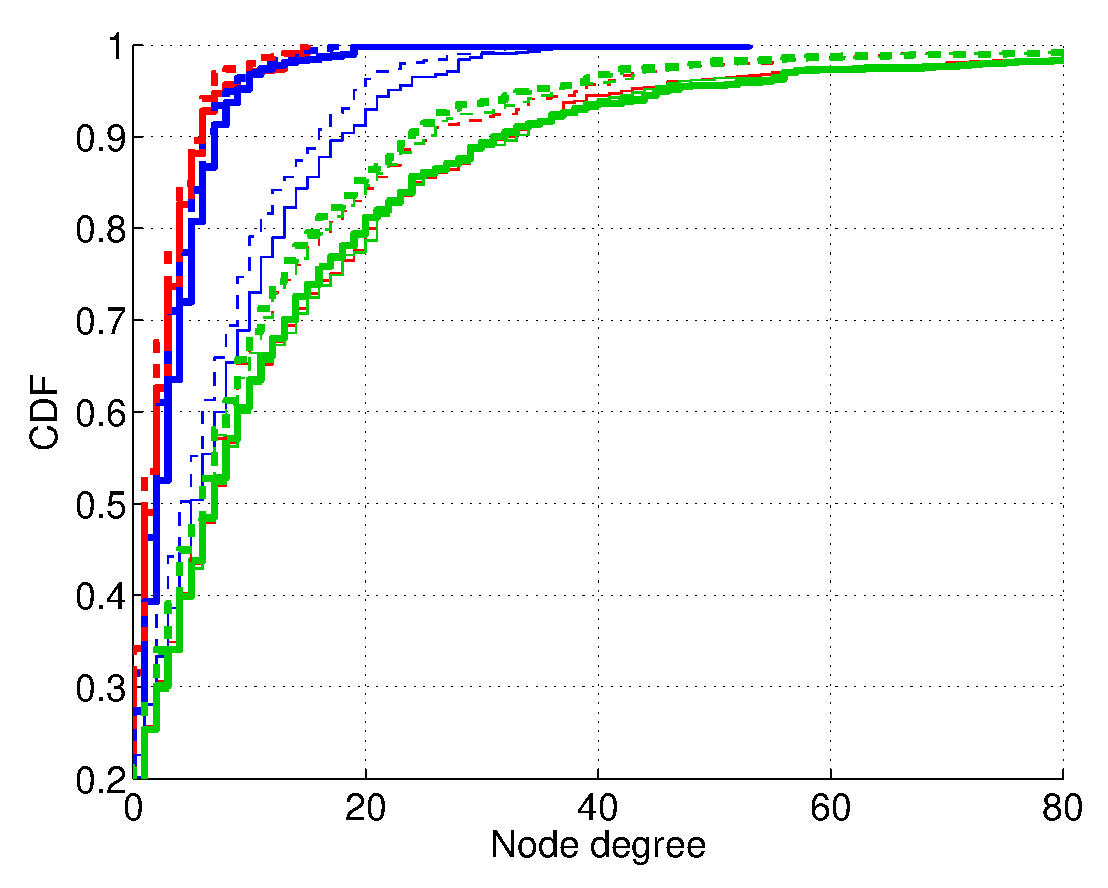
\includegraphics[width=.45\textwidth]{figures/cdf-first-node-degree.eps}\label{fig:cdf-first-node-degree}} \hfill
  \subfloat[TPD node degree]{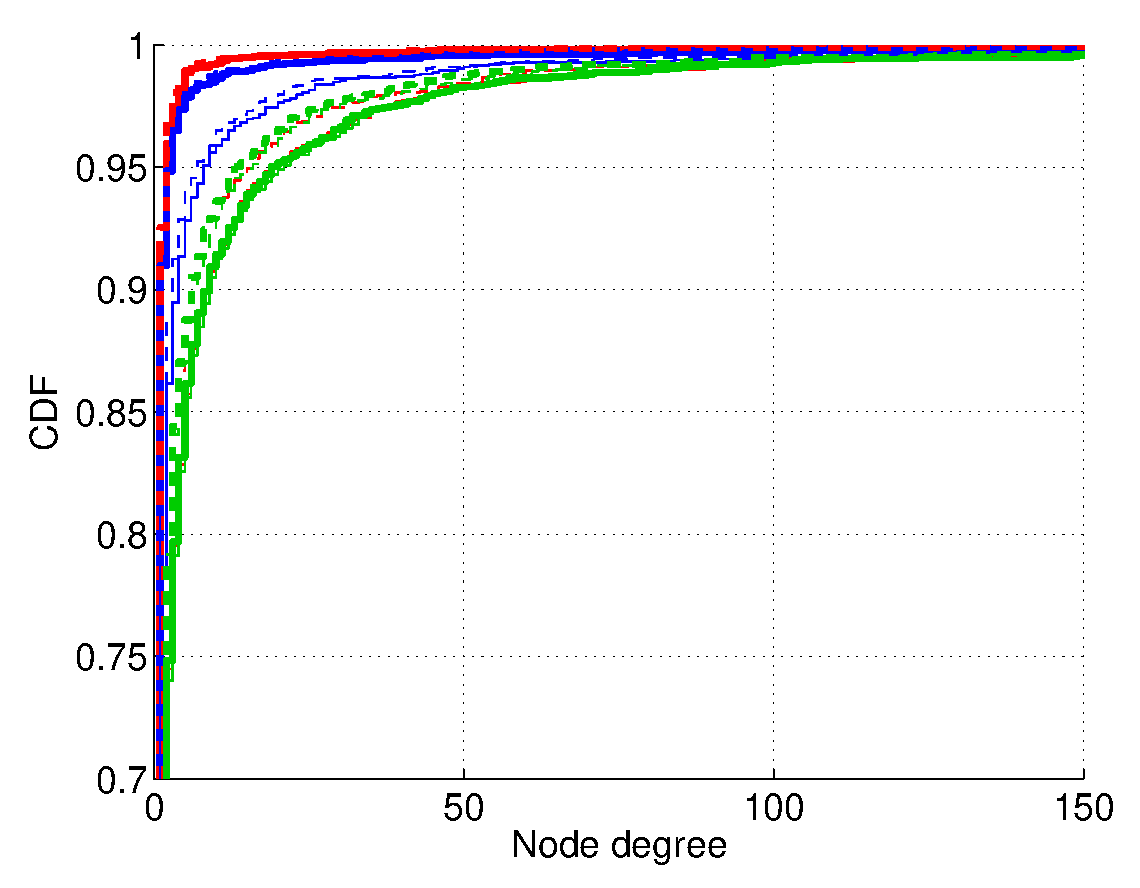
\includegraphics[width=.45\textwidth]{figures/cdf-third-node-degree.eps}\label{fig:cdf-third-node-degree}}
  
    \caption{CDF of FPD and TPD node degree for all browser profiles on 27/04/2016}
    \label{fig:cdf_first_third_node_degree}
\end{figure*}

\subsection{Graph separation}
\label{sec:graph_separation}
In order to investigate whether the ad-blocking tools have been subject to optimizations that would enable better filtering performances for the top-visited domains, our URL sample set $W$ includes, as explained in Section~\ref{sec:crawled_urls}, an additional set of 500 domains with a rank uniformly selected between 500 - 1M from the Alexa Top Rank. To this end, we separate the original graph $G$ into two independent graphs $G_T$ and $G_R$ for the 500 top-visited and the 500 uniformly-selected URLs, respectively, and followingly directly compare their filtering performances.

Figure~\ref{fig:top_last_domains_comparison} provides a comparison of the ad-blocking efficiency of the browser profiles $U$ for the two URL subsets. We observe that, the filtering performance of the different profiles remains roughly unaffected. We observe that Ghostery and AdblockPlus reduce the FPD node degree by an approximate factor of 5.7 and 4.3 for the top 500, while only 3.7 and 3 for the uniformly-selected 500 websites.

On one hand, this indicates a better filtering performance of Ghostery and AdblockPlus for the 500 top-ranked websites compared to the 500 uniformly-selected ones. On the other hand, Figure~\ref{fig:top_last_domains_comparison} shows that the mean FPD node degree of the 500 top-ranked websites ($\sim17$) is consistently and clearly higher than that of the 500 uniformly-selected websites ($\sim12$) without the use of any adblocker (profile \textit{NoAdblocker}). The 500 top-ranked websites therefore provide a larger margin for TPD node degree reduction or, equivalently, a bigger opportunity for improvement in terms of privacy.

To exemplify, supposed that a powerful adblocker could block all TPDs, its eventually measured filtering performance would be considerably higher for the 500 top-ranked URLs than for the 500 uniformly-selected ones.
Thenceforth, although a rank-oriented optimization of the adblockers seems a plausible assumption at a first glance, the different margins of improvement for the 500 top-ranked and the 500 uniformly-selected URLs do not allow us to judge whether adblockers are optimized for the top 500 websites or not.

\begin{figure*}[!t]
  \centering
  
  \subfloat[500 top-ranked FPDs]{\includegraphics[width=.45\textwidth]{figures/top500-first-means.eps}\label{fig:top500_first_means}} \hfill
  \subfloat[500 uniformly-selected FPDs]{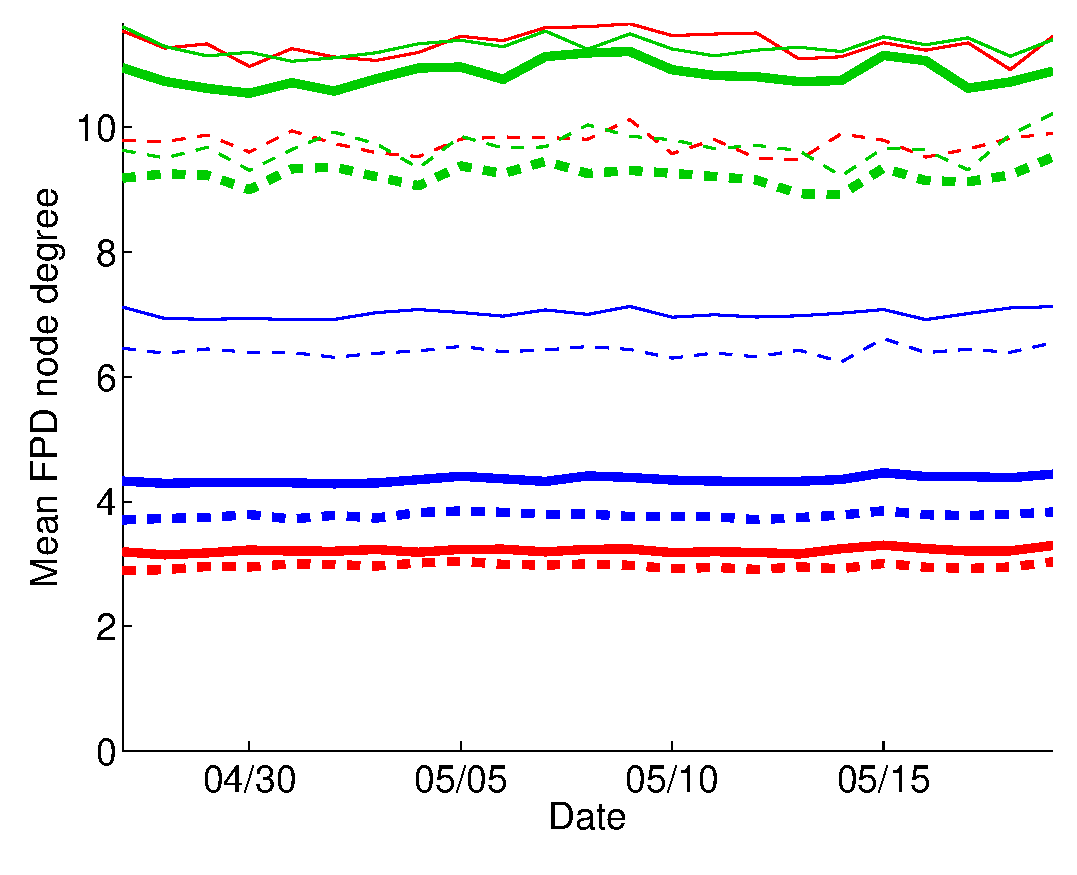
\includegraphics[width=.45\textwidth]{figures/last500-first-means.eps}\label{fig:top500_random_means}}
  
  \caption{Comparison of the mean FPD node degree of all browser profiles, separating the results for the top-visited domains and the uniformly-selected ones.}
  \label{fig:top_last_domains_comparison}
  \end{figure*}

\subsection{Relationship between rank and FPD node degree}
In this section we investigate the correlation between the Alexa rank of the URL and a filtering-performance metric ---i.e.\ the FPD node degree. In Figures~\ref{fig:first_party_degree_relative_rank_no_adblocker}, \ref{fig:first_party_degree_relative_rank_ghostery_max} and \ref{fig:first_party_degree_relative_rank_adblockplus_max} we plot the FPD node degree with respect to the domain rank to provide a finer visualization of the previous result, for the browser profiles \textit{NoAdblocker}, \textit{Ghostery\_\allowbreak MaxProtection} and \textit{Adblockplus\_\allowbreak MaxProtection}, respectively, on a specific date. The figures present only the data for the top 500-ranked websites.

Figure~\ref{fig:first_party_degree_relative_rank_no_adblocker} shows that, as we would expect, there exists a tendency for the higher-ranked domains to load more third parties, since the correlation between the rank and the FPD node degree is roughly 20\%. However, the browser profiles \textit{Ghostery\_\allowbreak MaxProtection} and \textit{Adblockplus\_\allowbreak MaxProtection} and do not show any trend that can suggest a clear relationship between the relative rank and the node degree. Our visual observation is confirmed by the calculation of the correlation of the two parameters that yields 2.15\% and 7.90\%, accordingly. This means that, albeit the higher-ranked domains tend to load more third parties, the use of the adblockers smooth these discrepancies, by reducing the node degree of the higher-ranked FPD nodes more than they do for the lower-ranked ones, as already discussed in \ref{sec:graph_separation}.

In order to investigate the effect of the rank on the CDF, we plot in Figure~\ref{fig:cdf_first_node_degree_no_adblocker} the results for the FPD nodes for (a) the total 1000 URLs, (b) the top-ranked 500 URLs and (c) the uniformly-selected ones, respectively. As can be seen, about 20\% of the websites loaded almost no third parties, while at the same time only a very limited number were accessed by more than 50 TPD nodes in all cases. Comparing the curves, we confirm that less third parties were loaded for the uniformly-selected domains, affirming the results of Figure~\ref{fig:top_last_domains_comparison}.

  \begin{figure*}
 \centering
 
 \subfloat[Scatterplot for \textit{NoAdblocker} with absolute correlation 19.87\%]{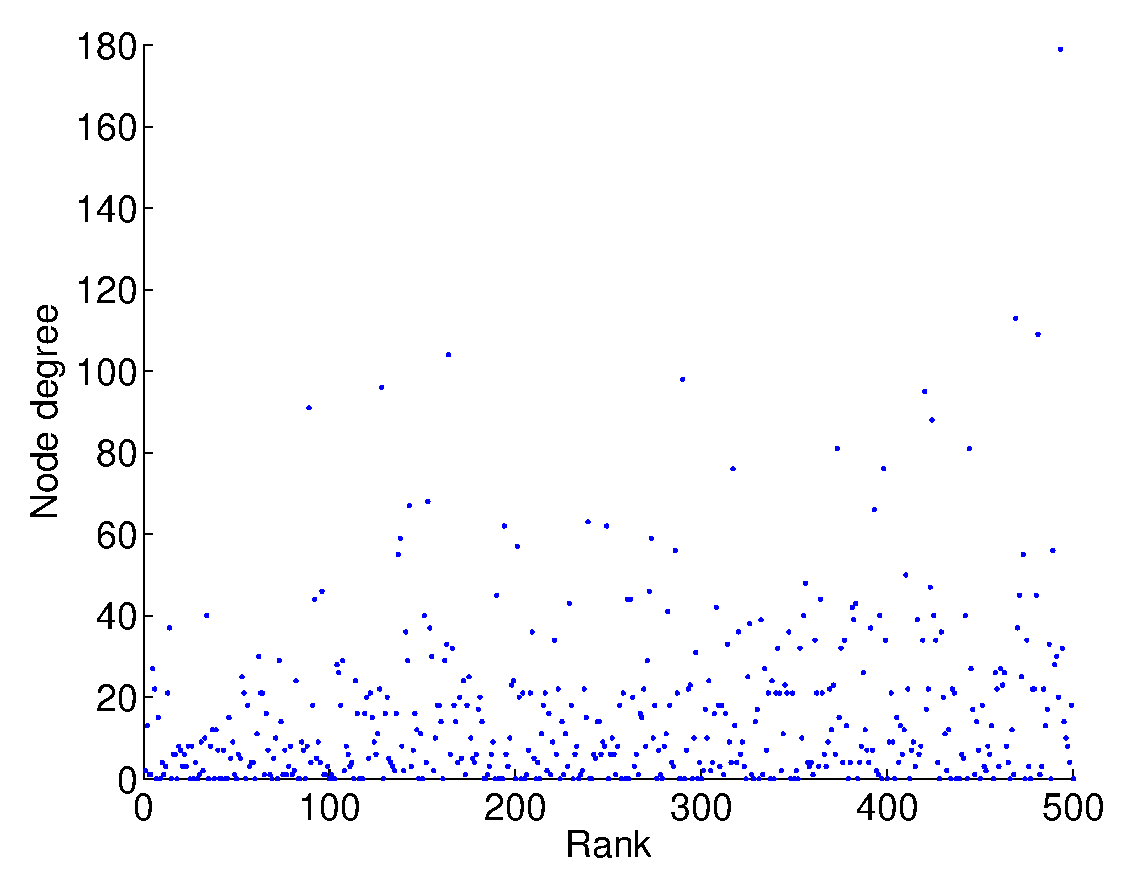
\includegraphics[width=.45\textwidth]{figures/scatterplot-fpd-no-adblocker.eps}\label{fig:first_party_degree_relative_rank_no_adblocker}} \hfill
 \subfloat[CDF for \textit{NoAdblocker}]{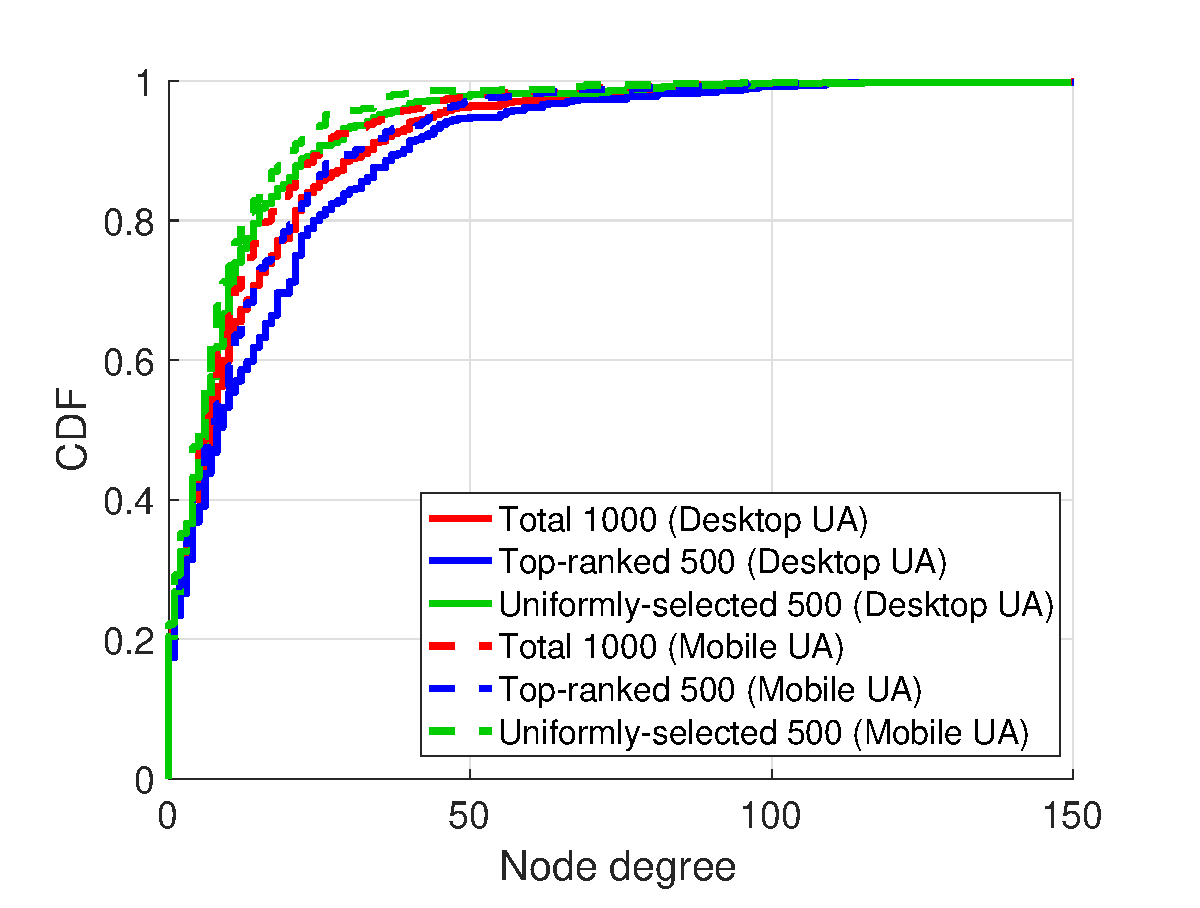
\includegraphics[width=.45\textwidth]{figures/comparative-cdf-first-node-degree-no-adblocker.eps}\label{fig:cdf_first_node_degree_no_adblocker}} \\
 \subfloat[Scatterplot for \textit{Ghostery\_\allowbreak MaxProtection} with absolute correlation 2.15\%]{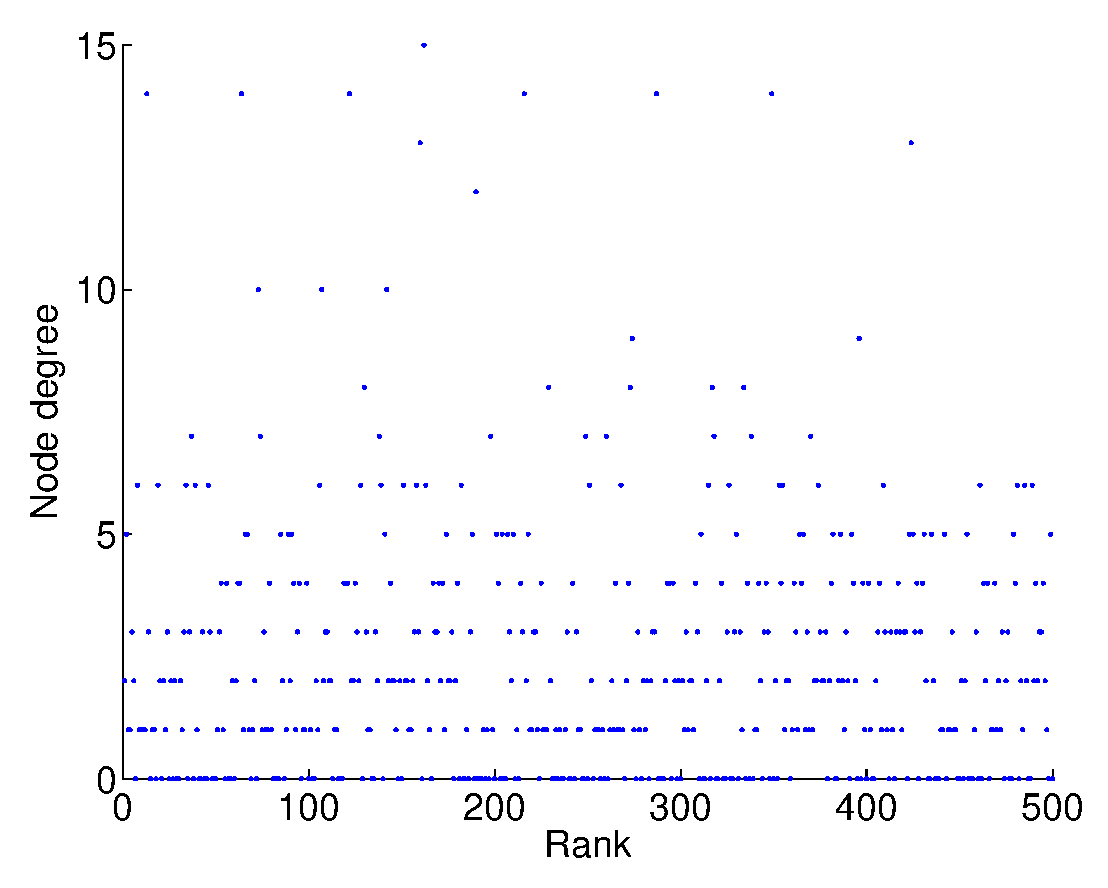
\includegraphics[width=.45\textwidth]{figures/scatterplot-fpd-ghostery-max.eps}\label{fig:first_party_degree_relative_rank_ghostery_max}} \hfill
 \subfloat[CDF for \textit{Ghostery\_\allowbreak MaxProtection}]{\includegraphics[width=.45\textwidth]{figures/comparative-cdf-first-node-degree-ghostery-max.eps}\label{fig:cdf_first_node_degree_ghostery_max}} \\
 \subfloat[Scatterplot for \textit{AdblockPlus\_\allowbreak MaxProtection} with absolute correlation 7.90\%]{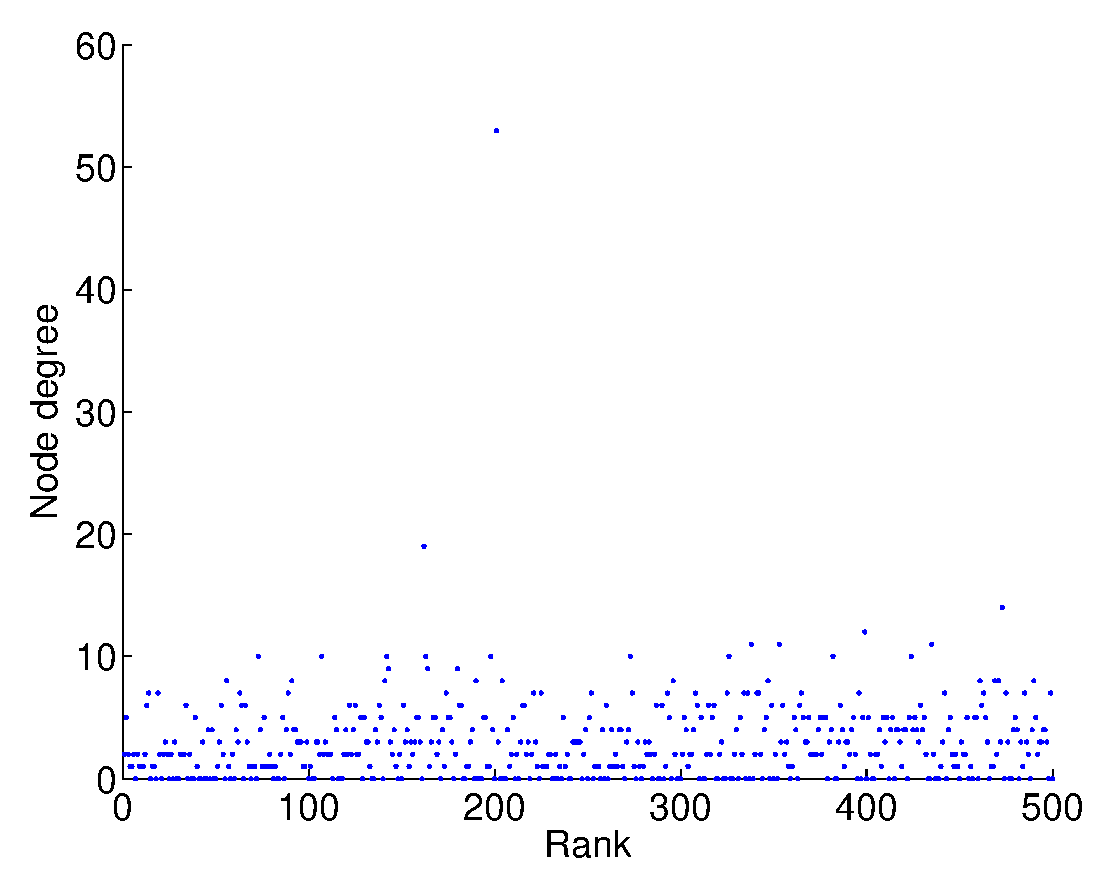
\includegraphics[width=.45\textwidth]{figures/scatterplot-fpd-adblockplus-max.eps}\label{fig:first_party_degree_relative_rank_adblockplus_max}} \hfill
 \subfloat[CDF for \textit{AdblockPlus\_\allowbreak MaxProtection}]{\includegraphics[width=.45\textwidth]{figures/comparative-cdf-first-node-degree-adblockplus-max.eps}\label{fig:cdf_first_node_degree_adblockplus_max}}
 
 \caption{\protect\subref{fig:first_party_degree_relative_rank_no_adblocker}, \protect\subref{fig:first_party_degree_relative_rank_ghostery_max}, \protect\subref{fig:first_party_degree_relative_rank_adblockplus_max} Scatterplot for the FPD node degrees of the 500 top-ranked domains and \protect\subref{fig:cdf_first_node_degree_no_adblocker}, \protect\subref{fig:cdf_first_node_degree_ghostery_max}, \protect\subref{fig:cdf_first_node_degree_adblockplus_max} CDF with separation of domains according to their ranks, for the browser profiles \textit{NoAdblocker}, \textit{Ghostery\_\allowbreak MaxProtection} and \textit{Adblockplus\_\allowbreak MaxProtection} on 20/05/2016}
 \label{fig:first_node_degree}
\end{figure*}

\subsection{Highest-degree domains}
In this section we focus particularly on the worst-case scenarios from a privacy viewpoint and present the degree of the first parties that load the highest number of third parties. To this end, we evaluate on a daily basis the top 1 (Figures~\ref{fig:first_mean_top1_without_entities},~\ref{fig:third_mean_top1_without_entities}) and top 10 domains (Figures~\ref{fig:first_mean_top10_without_entities},~\ref{fig:third_mean_top10_without_entities}) that load most third parties.

After an examination of the Figure~\ref{fig:highest_degree_nodes}, we observe that in the worst case, a first-party website can be tracked by up to 170 third parties (Figure~\ref{fig:first_mean_top1_without_entities}), while a third-party can have access and collect information about our browsing behavior from almost 500 first-party websites that we visited (Figure~\ref{fig:third_mean_top1_without_entities}). It is, however, important to mention that the filtering performances of the browser profiles $U$ remain approximately in the same relative order as in the previously analyzed cases, with the use of the adblockers to considerably enhance the user's protection against tracking.

Nevertheless, as expected, the results regarding the top 1 domain (Figures~\ref{fig:first_mean_top1_without_entities}, \ref{fig:third_mean_top1_without_entities}) present very high fluctuations, which are attenuated as we average over the top 10 websites (Figures~\ref{fig:first_mean_top10_without_entities}, \ref{fig:third_mean_top10_without_entities}). The plots are eventually considerably smoother when we average over 1000 websites (Figures~\ref{fig:first_means}, \ref{fig:third_means}).

    \begin{figure*}
   \centering
   
   \subfloat[Highest degree of FPD nodes for each day and browser profile $U$]{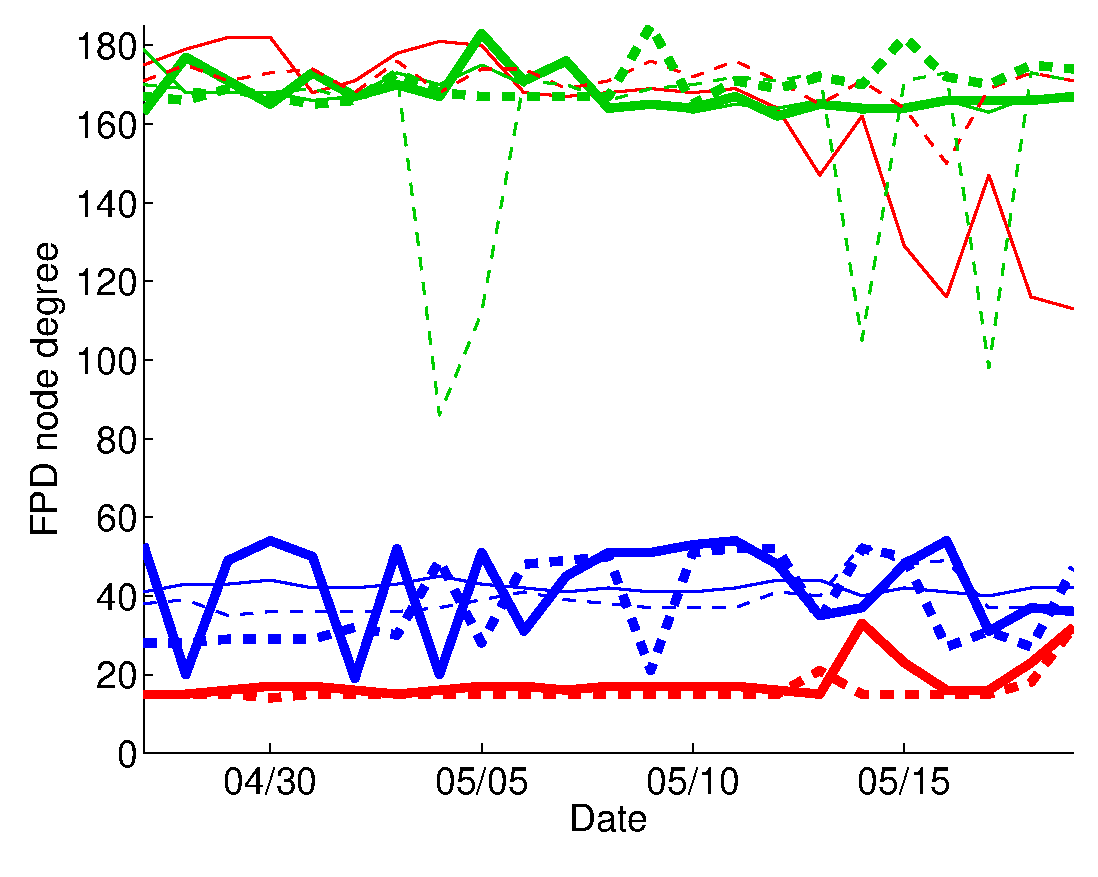
\includegraphics[width=.45\textwidth]{figures/first-mean-top1.eps}\label{fig:first_mean_top1_without_entities}} \hfill
   \subfloat[Mean value of the degree of the 10 most-connected FPD nodes for each day and browser profile $U$]{\includegraphics[width=.45\textwidth]{figures/first-mean-top10.eps}\label{fig:first_mean_top10_without_entities}} \\
   \subfloat[Highest degree of TPD nodes for each day and browser profile $U$]{\includegraphics[width=.45\textwidth]{figures/third-mean-top1.eps}\label{fig:third_mean_top1_without_entities}} \hfill
   \subfloat[Mean value of the degree of the 10 most-connected TPD nodes for each day and browser profile $U$]{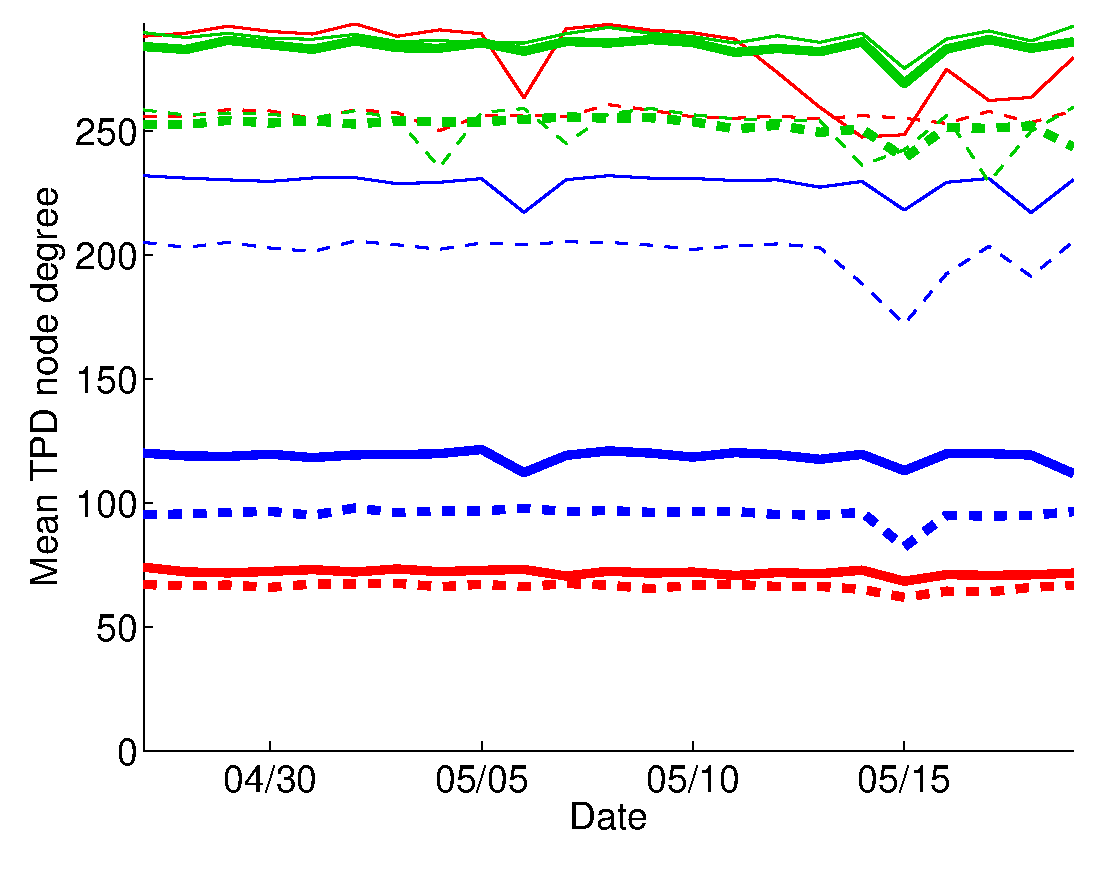
\includegraphics[width=.45\textwidth]{figures/third-mean-top10.eps}\label{fig:third_mean_top10_without_entities}}

  \caption{Time evolution of the first and third-party degree metrics for the most-connected FPD and TPD nodes, respectively}
  \label{fig:highest_degree_nodes}

  \end{figure*}

% \begin{figure}
%  \centering
%  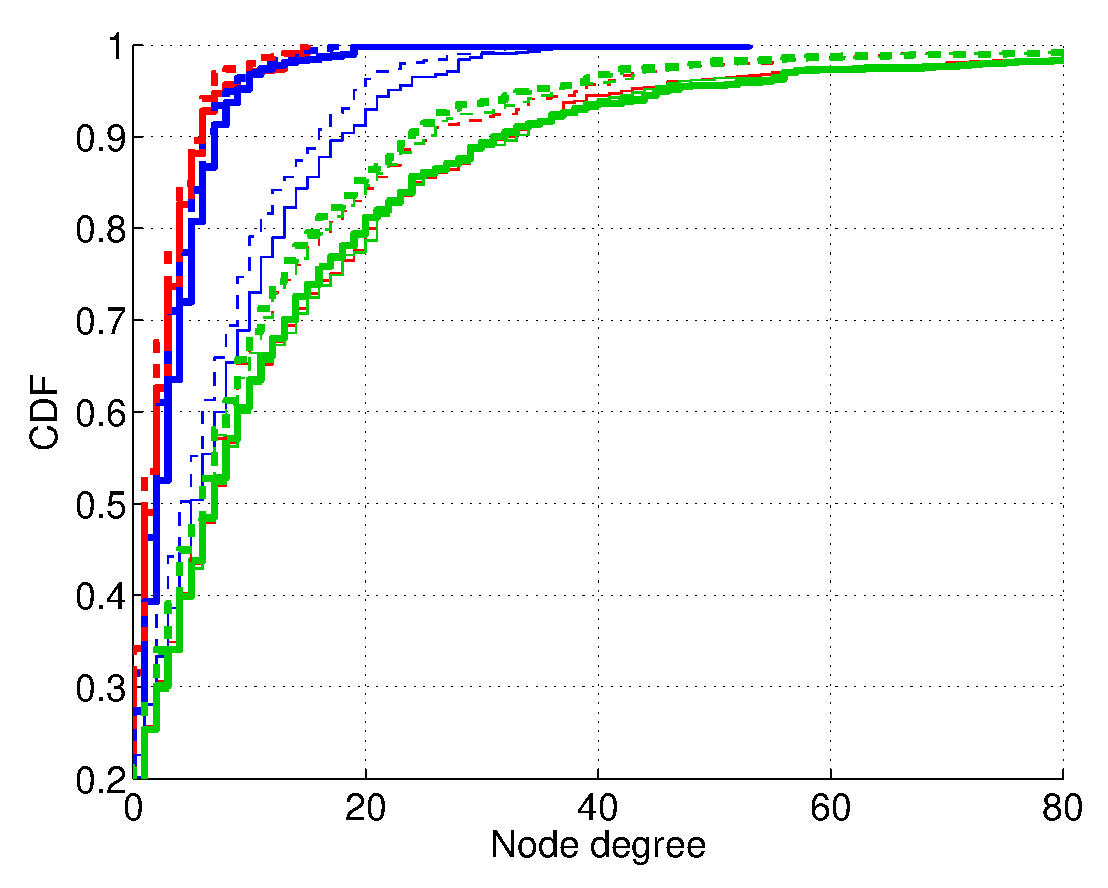
\includegraphics[width=.45\textwidth]{figures/cdf-first-node-degree.eps}
%  \caption{Cumulative distribution function of FPD node degree for the browser profile \textit{NoAdblocker} on 20/05/2016}
%  \label{fig:cdf_first_node_degree_no_adblocker}
% \end{figure}


\subsection{Metrics with entity grouping}
We now build the graphs $G_E$ that correspond to each browser profile $U$ by grouping multiple TPD nodes into one supernode representing their common administrative organization (legal entity) as described in Section~\ref{sec:legal_entity} and visualized in Figure~\ref{fig:graph}. We refer to this supernode as \textit{third-party entity} (TPE). Note that the FPDs remain unaltered in the new augmented graph. When we observe TPEs instead of TPDs, the mean FPD node degree is on the one hand reduced as an absolute number, while on the other hand, no considerable changes are to be observed for the mean TPE node degree or the graph density. As far as the relative ad-blocking efficiency of the browser profiles is concerned, we should remark that this does not present any change with respect to the results before entity grouping had been applied.

Comparing the mean FPD node degrees over time for the graphs $G$ (without entity grouping) in Figure~\ref{fig:metrics_without_entities} and $G_E$ (with entity grouping) in Figure~\ref{fig:metrics_with_entities} we observe that each visited URL from the sample set $U$ loads approximately 14 TPDs, but 12 TPEs on average. From graph $G$ we see that using AdblockPlus and Ghostery with maximal-protection configurations reduces the mean number of TPDs loaded by about 3.5 and 4.7 times, accordingly. Similarly, according to graph $G_E$ (Figure~\ref{fig:first_means_entities}), AdblockPlus and Ghostery reduce the mean number of TPEs loaded by roughly 3.4 and 4.8 times, respectively.

\begin{figure}
  \centering
  \subfloat[Mean FPD node degree]{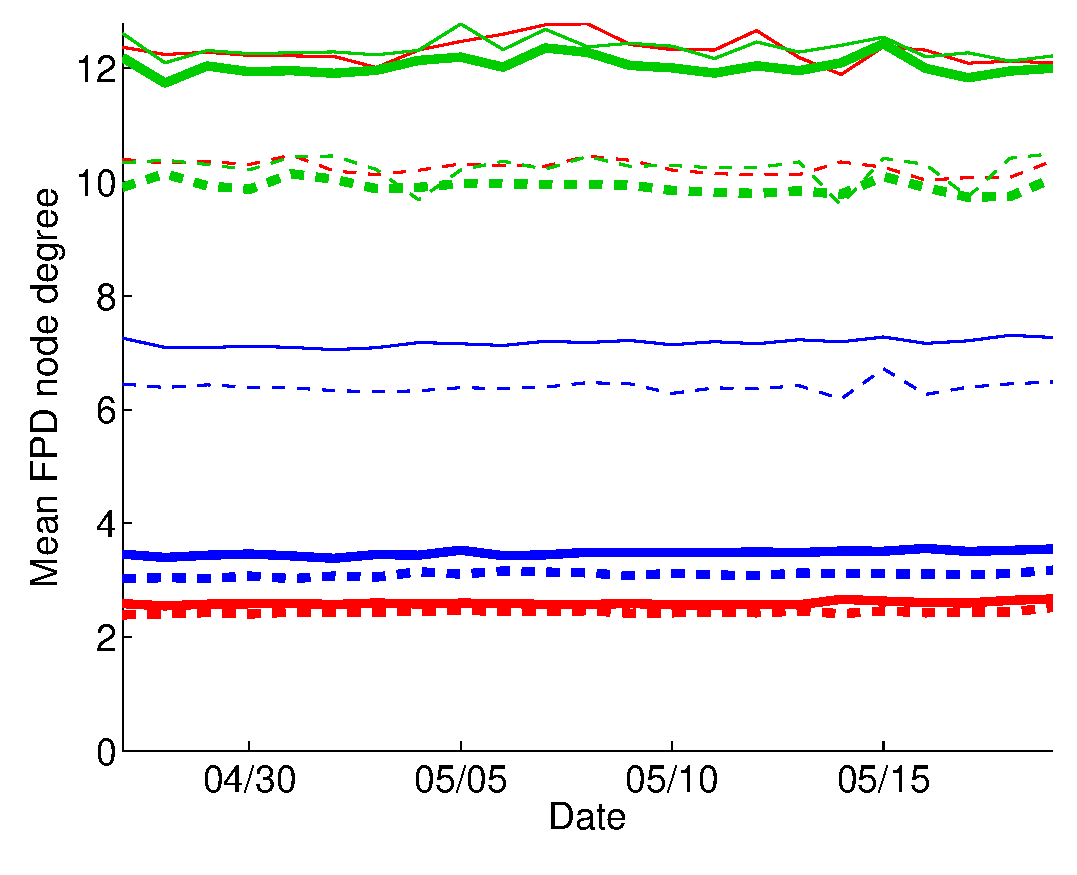
\includegraphics[width=.45\textwidth]{figures/first-means-entities.eps}\label{fig:first_means_entities}} \hfill
  \subfloat[Mean TPD node degree]{\includegraphics[width=.45\textwidth]{figures/third-means-entities.eps}\label{fig:third_means_entities}} \\
  \subfloat[Graph density]{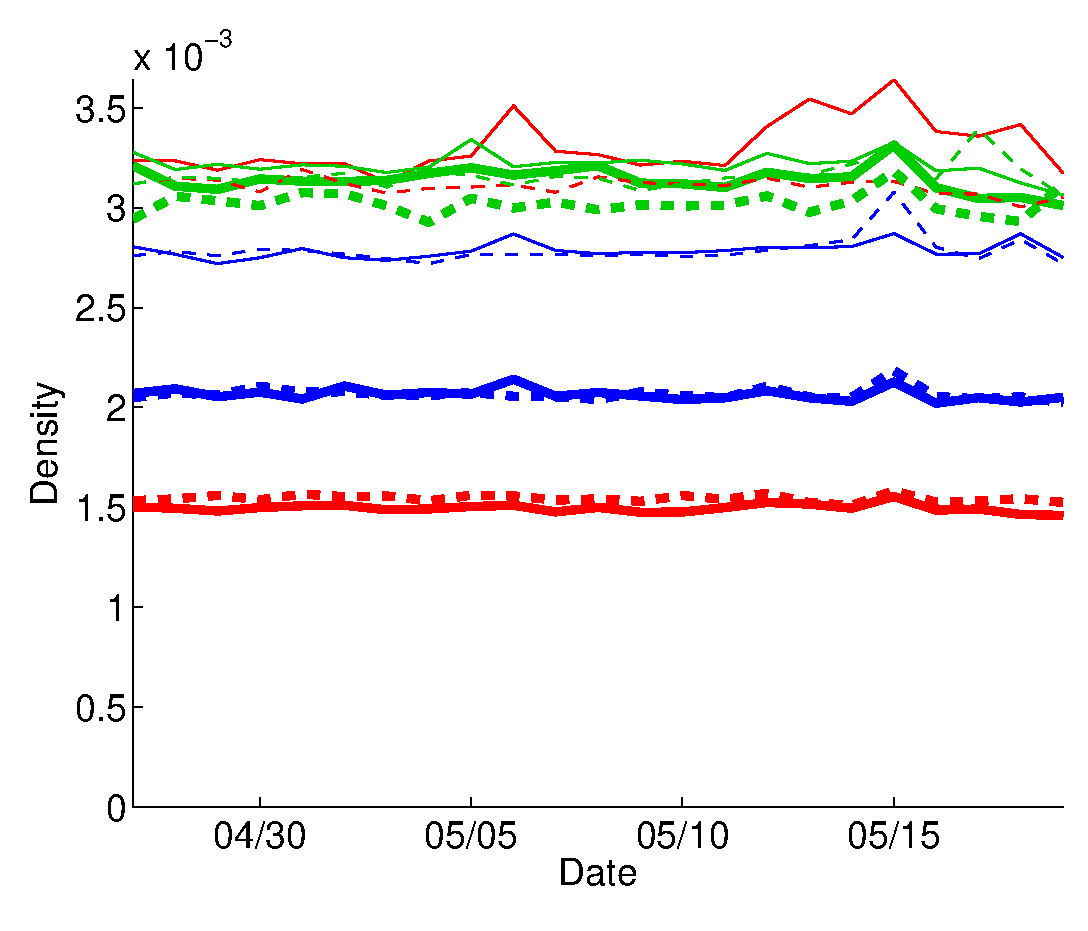
\includegraphics[width=.45\textwidth]{figures/density-entities.eps}\label{fig:density_entities}}

  \caption{Time evolution of graph metrics for all profiles \textbf{with} domain grouping according to entities}
  \label{fig:metrics_with_entities}
  \end{figure}



\section{Profile-parameter influence}
As explained in Chapter~\ref{sec:browser_profiles}, the browser profiles $U$ are created as a combination of different profile parameters under inspection. After a thorough examination of the experimental results of the previous sections, the impact of these parameters can be summarized as follows:

\vspace{0.5 em}\noindent \textbf{Adblocker installed:} Our results show that the use of an adblocker significantly reduces the number of third parties loaded by a factor of 40\% for an adblocker with default settings. By default Ghostery does not function as adblocker, while with maximum protection, Ghostery consistently outperforms AdblockPlus.

\vspace{0.5 em}\noindent \textbf{Block policy:} The block policy configured ---i.e. default or maximum protection--- for each adblocker results in a blocking difference of almost 80\% and 50\% for the mean first-party degree for Ghostery and AdblockPlus, respectively.

\vspace{0.5 em}\noindent \textbf{Do Not Track header:} The activation of the DNT flag has little impact on the results, since the browser user has no control over whether the DNT flag is honored or not and hence websites and advertisers may either obey or completely ignore it.

\vspace{0.5 em}\noindent \textbf{Mobile User Agent:} Websites that received requests by a mobile user agent indeed responded with a considerably lower number of third parties. A plausible explanation for this behavior is the requirement for less bandwidth that the mobile websites usually conform to. As a consequence of this limitation, less content is loaded and hence less requests are sent to third parties. This discrepancy was of course less obvious for the browser profiles with maximal protection enabled, since tracking by third parties is already reduced. To exemplify, in Figure~\ref{fig:third_means} the profiles \textit{Ghostery\_Default}, \textit{NoAdblocker} and \textit{NoAdblocker\_DNT} present a mean TPD node degree about 20\% higher than the corresponding browser profiles where a Mobile User Agent is used.

\subsection{Blacklist changes}
The different protection levels, \textit{Default} or \textit{MaxProtection}, for the two adblockers \textit{AdblockPlus} and \textit{Ghostery} respectively, are mainly achieved through the use of a different combination of blacklists. The blocking options of AdblockPlus are set through the direct inclusion of blacklists to be applied, while  Ghostery's blacklist configuration consists in the selection among a multitude of tracker categories to be blocked. An overview of these configurations is presented in Table~\ref{table:blacklists}.

Both adblockers store their blocking logic in the form of regular expressions of URLs and CSS rules, as explained in Chapter~\ref{sec:background}.

However, there is no metric that allows for comparison of regular expressions, thus making the direct comparison of the corresponding blacklists non quantifiable. Moreover, each entry in the blacklists does  not contribute equally to the blocking efficiency of the adblocker, since  some of the patterns are more often accessed than others, depending on the URL set that we crawl. Thence, adding or removing a URL pattern from a blacklist file does not necessarily imply an equal improvement or deterioration of the blacklist efficiency, accordingly.

As a consequence, by investigating the temporal changes of a blacklist file we cannot derive any robust privacy-comparison metric.

\begin{table*}
\centering
\begin{tabular}{|c|c c c c|}
\hline
\multirow{2}{*}{Protection Level} & \multicolumn{4}{|c|}{Lists} \\
& AdServers & EasyList & EasyListChina & EasyPrivacy \\
\hline
Default & & \checkmark & & \\
Maximal & \checkmark & \checkmark & \checkmark & \checkmark \\
\hline
\end{tabular}
\caption{AdblockPlus blacklist combination for default and maximal protection level. Ghostery's default and maximal protection correspond to the selection of none and all tracker categories, respectively.}
\label{table:blacklists}
\end{table*}


% \begin{figure}
%  \centering
%  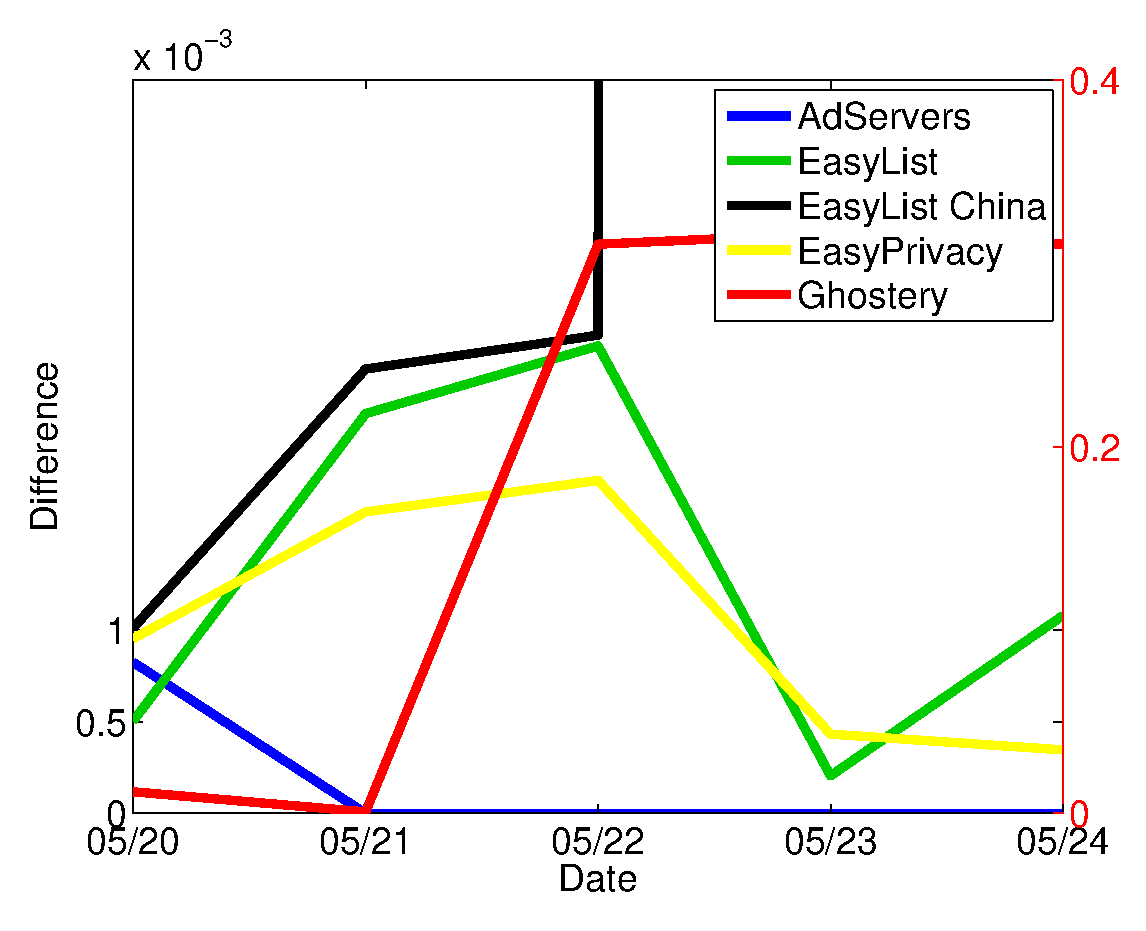
\includegraphics[width=.45\textwidth]{figures/blacklist-diff.eps}
%  \caption{Difference between a blacklist and its version on the previous day}
%  \label{fig:blacklist-diff}
% \end{figure}

\section{Geolocation of the legal entity of first-party and third-party domains}

Another interesting finding after the execution of our experiments and the entity analysis is the classification of the third parties according to their geographical location. With the entity data extracted from WHOIS, we use the matches between countries and third-party domains (TPD nodes) of the request graphs and visualize the comparison between the different countries on the world map in Figure~\ref{fig:third_party_entity_map}. The darkest regions (red) are the countries with the most TPEs loaded, while the white ones host none of the TPEs found in our graphs. As we would expect, the USA host by far most of the third-party domains loaded, while the rest of the countries account for a considerably lower percentage of TPEs.

Note that only a part of the TPDs ---accounting for about 60\%--- could be assigned to a TPE and followingly to a country. One reason is that WHOIS does not provide sufficient information for all of the TPDs loaded. Moreover, the script that allowed for the automated extraction of the entity information depends on a relatively uniform format of the WHOIS documents and as a result, deviations from this format will cause information loss.

A more detailed view of the number of TPEs hosted by the top 10 countries is presented in Table~\ref{table:top_10_third_party_countries}. For each row, the absolute numbers refer to the TPDs that were recognized and assigned to a TPE for the specific country, while the percentages refer to the ratio of these TPEs over the total number of TPEs that were recognized by our automated script. In this table, we compare the TPEs hosted by each of these countries (column \textit{None}) to the number of TPEs loaded when the adblockers Ghostery and AdblockPlus are deployed under maximum-protection settings (columns \textit{Ghostery} and \textit{AdblockPlus}).

Similarly, the USA host most of the legal entities of the FPDs visited, as results from Table~\ref{table:top_10_first_party_countries} that lists the countries and the number of first-party legal entities (FPEs) that reside in them. The heat map in Figure~\ref{fig:first_party_entity_map} summarizes in a similar manner the countries and the corresponding number of FPEs hosted in them.

Unsurprisingly, the results do not present any considerable deviation from the conclusions we extracted for the TPEs: The USA hosts roughly 36\% of the FPEs and is followed by Canada that only hosts about 7\% of them. On the other extreme, South American and African countries host very few FPEs, as we already observed in the heat maps corresponding to the third parties (Figure~\ref{fig:third_party_map}).

\begin{table}
  \centering
  \begin{tabular}{|c|c|c|c|}
  \hline
  \multirow{2}{*}{Country} & \multicolumn{3}{|c|}{Third-Party Entities} \\
  \cline{2-4}
  & \scriptsize{None} & \scriptsize{Ghostery} & \scriptsize{AdblockPlus} \\
  \hline
  United States & 784 (45\%) & 483 (42\%) & 500 (45\%) \\
  Germany & 106 (6\%) & 40 (4\%) & 34 (3\%) \\
  China & 82 (5\%) & 70 (6\%) & 67 (6\%) \\
  Japan & 80 (5\%) & 62 (5\%) & 61 (6\%) \\
  Great Britain & 77 (4\%) & 43 (4\%) & 44 (4\%) \\
  France & 69 (4\%) & 33 (3\%) & 31 (3\%) \\
  Canada & 49 (3\%) & 33 (3\%) & 28 (3\%) \\
  India & 46 (3\%) & 38 (3\%) & 38 (3\%) \\
  Panama & 41 (2\%) & 32 (3\%) & 25 (2\%) \\
  Turkey & 32 (2\%) & 27 (2\%) & 27 (2\%) \\
  \hline
  Total & 2908 & 1866 & 1812 \\
  Found & 1748 (60.1\%) & 1140 (61.1\%) & 1097 (60.5\%) \\
  \hline
  \end{tabular}
  \caption{Countries hosting the highest percentage TPEs when no adblocker is used (browser profile \textit{NoAdblocker}), and the corresponding percentages when Ghostery and AdblockPlus are used under maximum protection settings (browser profiles \textit{Ghostery\_MaxProtection} and \textit{Adblockplus\_MaxProtection}) on 28/04/2016.}
  \label{table:top_10_third_party_countries}
  \end{table}
  
  \begin{table}
  \centering
  \begin{tabular}{|c|c|}
  \hline
  Country & First-Party Entities \\
  \hline
  United States & 35.7 \% \\
  Canada & 7.4 \% \\
  Japan & 4.8 \% \\
  Switzerland & 4.0 \% \\
  Germany & 3.8 \% \\
  India & 3.5 \% \\
  Great Britain & 3.0 \% \\
  Russia & 2.6 \% \\
  France & 2.6 \% \\
  Panama & 2.0 \% \\
  \hline
  \end{tabular}
  \caption{Countries hosting the highest percentage First-Party Entities}
  \label{table:top_10_first_party_countries}
  \end{table}
  

\begin{figure*}[!t]
 \centering
 
  \subfloat[Third-party legal entity locations]{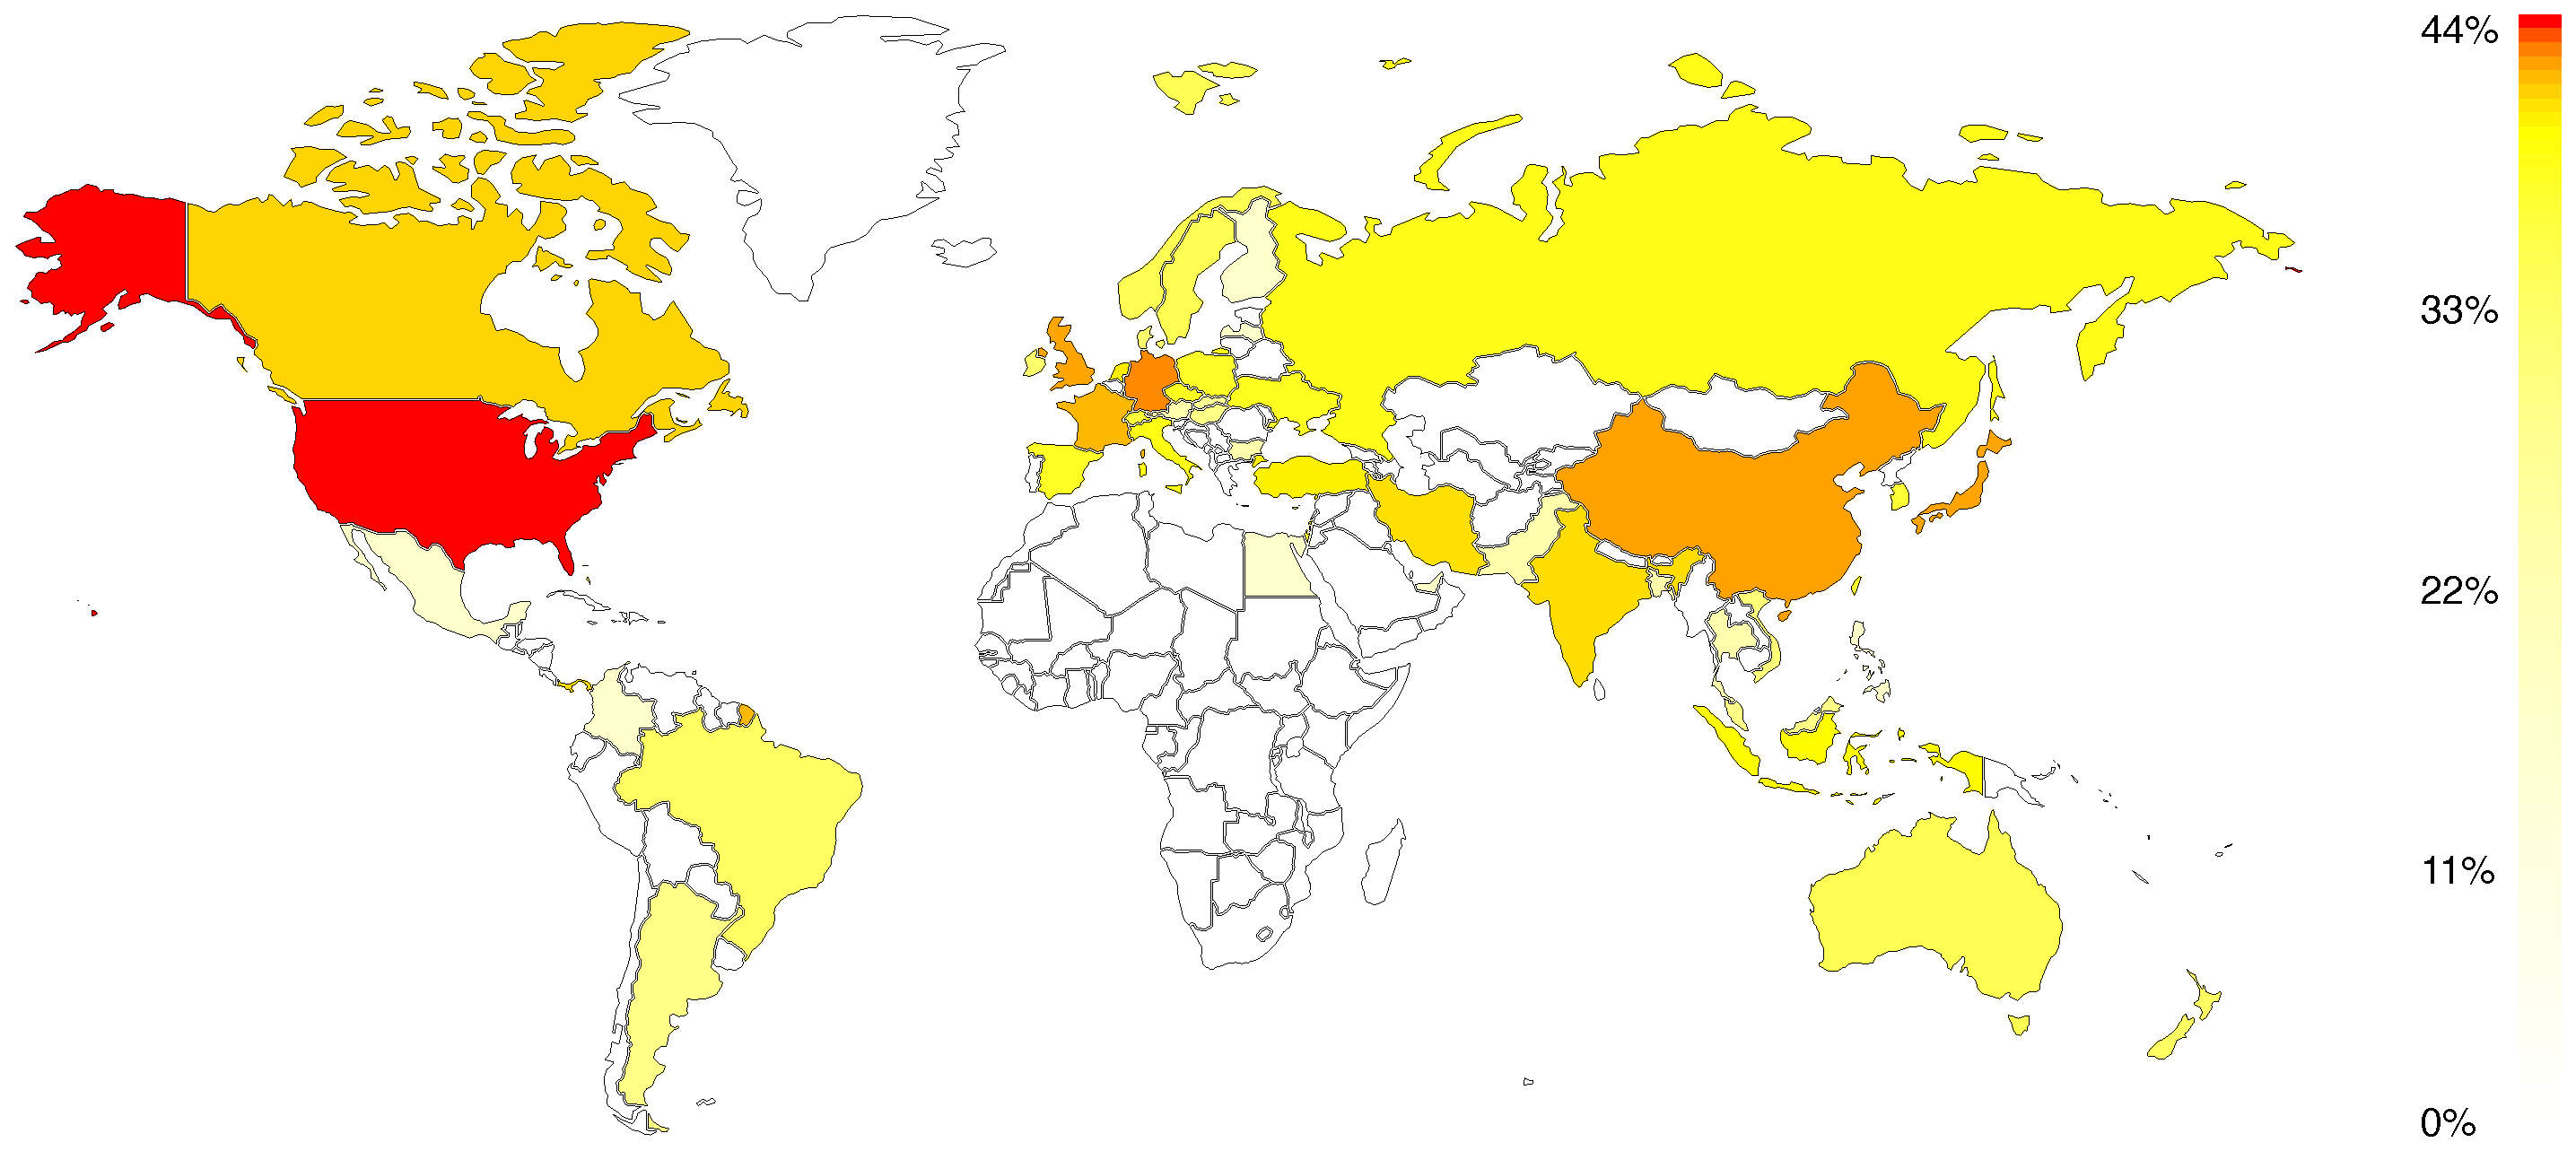
\includegraphics[width=\textwidth]{figures/third_party_entity_map.eps}\label{fig:third_party_entity_map}} \hfill
  \subfloat[Third party server locations]{\includegraphics[width=\textwidth]{figures/third_party_server_map.eps}\label{fig:third_party_server_map}}
 
 \caption{World map depicting the locations of the legal entities and the servers for the third parties loaded during our experiments.}
 \label{fig:third_party_map}
\end{figure*}

\begin{figure*}
    \centering
    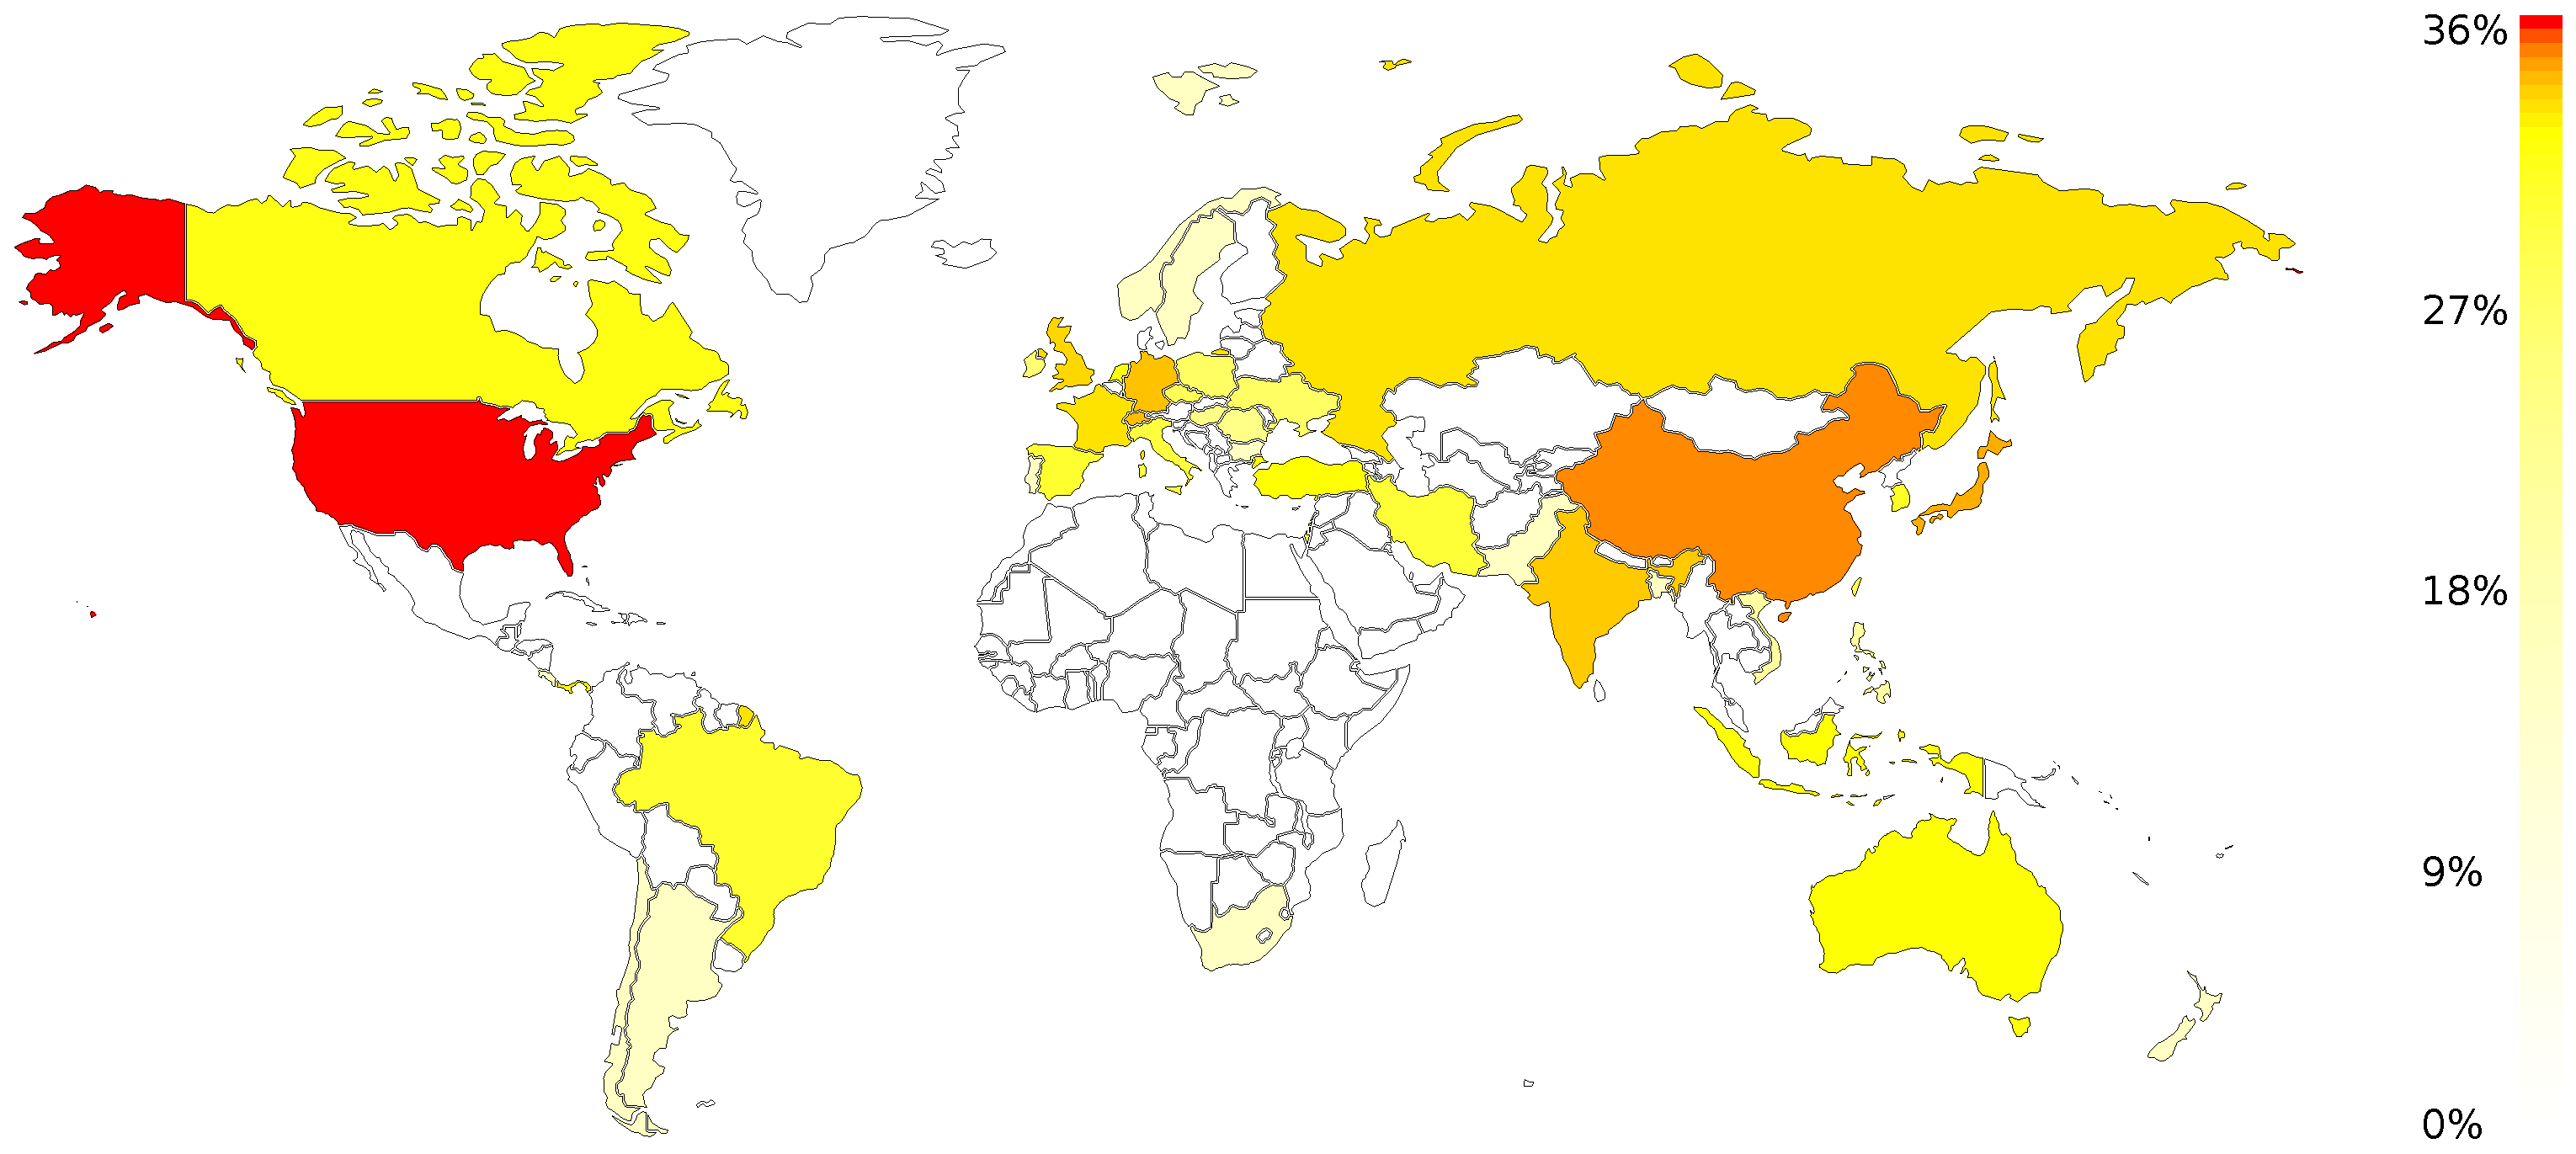
\includegraphics[width=\textwidth]{figures/first_party_entity_map.eps}
    \caption{World map depicting the locations of the legal entities for the first parties visited during our experiments}
    \label{fig:first_party_entity_map}
\end{figure*}

\section{Legal entity}
After the examining of the graph metric results without entity grouping (Figure~\ref{fig:metrics_without_entities}) and comparing them to the results with entity grouping (Figure~\ref{fig:metrics_with_entities}), we conclude that grouping the TPD nodes according to the legal entities they belong to brings a considerable reduction of the mean FDP node degree, asserting that the number of legal entities potentially collecting information about the user is indeed less than that of the actual third-party domains tracking them.

On the contrary, the mean TPD node degree, as well as the graph density do not present any significant variation, which leads us to the conclusion that the various legal entities have on average access to roughly the same first parties, although controlling multiple third-party domains.

Table~\ref{table:top_10_tpd_entities} summarizes the 10 entities with the highest TPD node degree, i.e.\ that were present on most of the visited URLs when the default Browser settings were applied (\textit{NoAdblocker}) and for a specific date. As the data suggests, \textit{Google Inc.} is loaded by 674 out of the 1000 URLs visited, thus having the most frequent presence among the rest of the third-party entities. The relative presence among the entities can be directly compared by their normalized degree, that is, the FPD node degree of the entity divided by the maximum FPD node degree found in our experiments ---in this case the degree of the entity \textit{Google Inc.}.

Analogous results are extracted from Table~\ref{table:top_10_third_party_domains} that lists the 10 domains with the highest TPD node degree. More specifically, 7 out of 10 of these TPDs belong to the same legal entity, i.e. \textit{Google Inc.}. The two other entities that appear in the list are \textit{Facebook Inc.} and \textit{AppNexus Inc.}, thus confirming the results the Table~\ref{table:top_10_tpd_entities}, where the three first places are occupied by the exact same legal entities.

\begin{table}
  \centering
  \begin{tabular}{|c|c|c|c|c|}
  \hline
  \multirow{2}{*}{Legal Entity} & \multicolumn{3}{|c|}{Degree} \\
  \cline{2-4}
    & \scriptsize{None} & \scriptsize{Ghostery} & \scriptsize{AdblockPlus} \\
  \hline
  Google Inc. & 666 & 328 & 354 \\
  Facebook Inc. & 328 & 6 & 211 \\
  AppNexus Inc. & 159 & 0 & 0 \\
  TMRG Inc. & 143 & 0 & 4 \\
  Twitter Inc. & 137 & 9 & 87 \\
  Oracle Corporation & 123 & 2 & 39 \\
  Adobe Systems Incorporated & 107 & 6 & 32 \\
  Yahoo! Inc. & 99 & 7 & 5 \\
  AOL Inc. & 88 & 3 & 3 \\
  OpenX Technologies & 88 & 0 & 0 \\
  \hline
  \end{tabular}
  \caption{Legal entities with the highest TPE node degree for browser profile \textit{NoAdblocker} and the corresponding values for Ghostery and AdblockPlus with maximum-protection settings (browser profiles \textit{Ghostery\_MaxProtection} and \textit{AdblockPlus\_MaxProtection}) on 28/04/2016.}
  \label{table:top_10_tpd_entities}
  \end{table}
  
  \begin{table}
  \centering
  \begin{tabular}{|c|c|c|c|c|c|}
  \hline
    \multirow{2}{*}{Third-Party Domain} & \multirow{2}{*}{Legal Entity} & \multicolumn{3}{|c|}{Degree} \\
  \cline{3-5}
    & & \scriptsize{None} & \scriptsize{Ghostery} & \scriptsize{AdblockPlus} \\
  \hline
  doubleclick.net & Google Inc. & 486 & 0 & 1 \\
  google-analytics.com & Google Inc. & 476 & 4 & 0 \\
  google.com & Google Inc. & 383 & 93 & 144 \\
  facebook.com & Facebook Inc. & 318 & 5 & 164 \\
  gstatic.com & Google Inc. & 308 & 226 & 235 \\
  googlesyndication.com & Google Inc. & 204 & 0 & 0 \\
  google.ch & Google Inc. & 189 & 0 & 0 \\
  fonts.googleapis.com & Google Inc. & 185 & 145 & 141 \\
  adnxs.com & AppNexus Inc. & 159 & 0 & 0 \\
  facebook.net & Facebook Inc. & 157 & 0 & 140 \\
  \hline
  \end{tabular}
  \caption{Top-loaded TPDs for browser profile \textit{NoAdblocker} and the corresponding values for Ghostery and AdblockPlus with maximum-protection settings (browser profiles \textit{Ghostery\_MaxProtection} and \textit{AdblockPlus\_MaxProtection}) on 28/04/2016}
  \label{table:top_10_third_party_domains}
  \end{table}

\section{Rank impact}

In Figures~\ref{fig:top_last_domains_comparison} and~\ref{fig:cdf_first_node_degree_no_adblocker} we investigated the relationship between the URL rank and the FPD node degree.

As resulted from the plot of the mean FPD node degree (Figure~\ref{fig:top_last_domains_comparison}), the uniformly-selected FPD nodes were accessed on average by less third parties with respect to the top-ranked 500 FPD nodes, thus contradicting our initial assumption. On the other hand, a higher number of loaded third parties can be justified, if the size and the popularity of the first domains is taken into consideration, as opposed to that of the last domains.

Another observation can be made when the correlation between the rank and the FPD node degree is examined. More specifically, the rank of each website among the top 500 of the rank (Figure~\ref{fig:first_party_degree_relative_rank_no_adblocker}) does not present a strong correlation to the number of third parties it loaded, hence reinforcing our conclusion above.